\documentclass[sn-basic,Numbered]{sn-jnl}

% ── Packages ────────────────────────────────────────────────────────────────
\usepackage{amsmath,amsfonts}
\usepackage{graphicx}
\usepackage{hyperref}
\usepackage{float}
\usepackage{booktabs}
\usepackage{tikz}
\usepackage{array}
\usepackage{tabularx}
\usepackage{pgfplots}
\usepackage{lscape}
\usepackage{rotating}
\usepackage{multirow}
\usepackage{makecell}
\usepackage{longtable}
\usepackage{ragged2e}
\newlength{\tblw}
\setlength{\tblw}{\dimexpr\textwidth-12\tabcolsep-7\arrayrulewidth\relax}

% sn-jnl leaves \cline undefined (it does \let\cline\cmidrule before \cmidrule
% exists). Restore the standard LaTeX/array definition.
\makeatletter
\let\cline\@undefined
\newcommand*\cline[1]{\@cline#1\@nil}
\makeatother

% Proportional-width X columns for tabularx (replaces \resizebox on tables)
\newcolumntype{Y}[1]{>{\hsize=#1\hsize\linewidth=\hsize\raggedright\arraybackslash}X}
\pgfplotsset{compat=1.18}
\usetikzlibrary{shapes.geometric, arrows.meta, positioning, calc}

% ── Document ─────────────────────────────────────────────────────────────────
\begin{document}

% ── Title ────────────────────────────────────────────────────────────────────
\title{AI for Scientific Research: A Comprehensive
Survey on Architecture, Research Lifecycle
Integration, Ethics and Security}

% ── Authors ─────────────────────────────────────────────────────────────────
\author[1]{\fnm{Balaji Prabhu} \sur{B V}}\email{bvb@mcehassan.ac.in}

\author[1]{\fnm{Mohammed} \sur{Zaid}}\email{mohammedzaid.msajid@gmail.com}

\author[1]{\fnm{Jayasaham} \sur{ND}}\email{shamnd0919@gmail.com}

\author[1]{\fnm{Lohith} \sur{G}}\email{lohith15.g@gmail.com}

\author[1]{\fnm{Keerthan} \sur{KM}}\email{keerthankm07@gmail.com}

\author*[2]{\fnm{Shrishma Rao} \sur{V S}}\email{shrishma.rao@manipal.edu}

\affil*[1]{\orgname{Malnad College of Engineering}, \city{Hassan}, \state{Karnataka}, \country{India}}

\affil*[2]{\orgname{Manipal Academy of Higher Education}, \city{Manipal}, \state{Karnataka}, \country{India}}

% ── Abstract ─────────────────────────────────────────────────────────────────
\abstract{Scientific literature is growing fast and research workflows are getting more complicated, so demand for AI tools that help at each stage of scholarly work is rising. Existing surveys usually cover a single task, such as literature retrieval, or describe agent architectures without tying them to the research lifecycle. We address that gap with a systematic review of 40 peer-reviewed journal papers, conference papers, and preprints published from 2019 to 2026 (see Section~\ref{sec:methodology}). The review asks how AI systems are designed, deployed, and evaluated across the research workflow, from topic exploration and literature review through experimentation, writing, peer review, and governance. Using a coding methodology based on PRISMA 2020, we group the literature into four themes: research guidance and lifecycle integration, agentic and retrieval-augmented architectures, tool ecosystems, and ethics and security. Hybrid modular architectures, which combine retrieval-augmented generation, multi-agent coordination, and human oversight, are more often reported to outperform monolithic or fully autonomous designs. That pattern rests on qualitative comparisons inside individual primary studies. No controlled, head-to-head benchmark compares the architectures directly. The corpus also points to four research gaps: there are no standardized end-to-end benchmarks, factual grounding in multi-step workflows is unresolved, long-horizon memory and cross-document reasoning are underdeveloped, and explainability and auditability are limited. We then propose an architectural-lifecycle framework that maps six research-lifecycle stages against the four levels of the agent-architecture taxonomy developed in this survey. Section~\ref{sec:introduction} explains how it differs from prior surveys. The review follows PRISMA 2020 \cite{page2021prisma}, with the checklist and search-and-screening details in Section~\ref{sec:methodology}. We did not pre-register a protocol, since this is a structured academic survey and not a clinical systematic review.}

\keywords{AI in Scientific Research, Automated Literature Review, Research
Automation, Research Agents, Scientific Writing Assistance, Paper
Summarization, Scientific Document Analysis, Scholarly Data Processing,
AI Ethics in Research}

\maketitle

\let\thefootnote\relax\footnotetext{The authors declare no conflict of interest.}

% ════════════════════════════════════════════════════════════════════════════
\section{Introduction}
\label{sec:introduction}
% ════════════════════════════════════════════════════════════════════════════

Artificial intelligence is moving from isolated task automation toward
systems that take part in broader research workflows. In scholarly
settings, the growing volume of publications, the complexity of
disciplinary knowledge, and the demand for faster synthesis have made
manual literature processing harder to sustain. As a result, AI now
supports individual subtasks including fuller research processes,
topic discovery, literature review, evidence extraction,
scientific writing, and review support
\cite{vishnumolakala2024arc,lian2025literature,bolanos2024ailitreview}.

A recurring theme in the literature is AI emerging as a research
companion. Systems such as ARC help students identify suitable topics and organize early-stage
research activity \cite{vishnumolakala2024arc}. Other systems focus on
literature mining, paper screening, and structured extraction of
experimental knowledge from scientific texts
\cite{lian2025literature}. A third line of work automates parts of
systematic literature review workflows while leaving final inclusion,
interpretation, and synthesis decisions to humans
\cite{bolanos2024ailitreview}. Together, these studies suggest AI is
becoming a working part of the research lifecycle.

This survey addresses a gap in the literature by organizing these
developments into a coherent architectural and lifecycle-based
framework. Prior surveys cover narrower ground: Bola\~nos et al.\
\cite{bolanos2024ailitreview} focus only on literature review
automation, Gridach et al.\ \cite{gridach2025scientific} examine
agentic discovery without addressing governance, and Chen et al.\
\cite{chen2025ai4research} survey AI4Research tasks without an
architectural taxonomy. This work spans the full research lifecycle,
integrates architectural analysis with lifecycle coverage, and treats
ethics and security as design constraints rather than afterthoughts.
This survey is built around four research questions:
\begin{itemize}
\item \textbf{RQ1.} How is AI currently used across the stages of the scientific research lifecycle, from topic exploration through peer review and governance, and how mature is each application area (Section~\ref{sec:useofai})?
\item \textbf{RQ2.} What architectural patterns underlie research-oriented AI agents, and how do component techniques, agent patterns, operational-management layers, and deployment-scale architectures trade off against each other (Section~\ref{sec:architectures})?
\item \textbf{RQ3.} Within the reviewed corpus, does the evidence favor monolithic or hybrid modular agent architectures for scholarly tasks (Section~\ref{sec:architectures})?
\item \textbf{RQ4.} What gaps in evaluation, grounding, memory, and auditability limit how far research AI agents can be trusted, and what design directions follow from them (Section~\ref{sec:gaps})?
\end{itemize}
In answering these questions, the survey makes five differentiated contributions:

\begin{enumerate}
  \item \textbf{Unified lifecycle taxonomy.} We map 40 papers onto a six-stage research lifecycle (Section~\ref{sec:useofai}). We keep the sequential stages analytically distinct from cross-cutting support activities (e.g., funding) and research-method categories (e.g., qualitative-research tooling), and for each stage we note which AI capabilities are mature, which are emergent, and which remain unsupported. This gives more complete coverage than the single- or dual-task framing used in prior surveys.

  \item \textbf{Architectural taxonomy with trade-off analysis.} We compare twelve agent architecture families, from classical reactive models through Agentic RAG, TacTool, and AgentOps, and assess their suitability for scholarly use cases. Gridach et al.\ and AI4Research offer descriptive inventories; we go further and weigh the trade-offs between families.
\item \textbf{Expanded tool ecosystem review.} We evaluate twelve AI research tools, against three in most prior surveys, covering both discovery-oriented platforms and synthesis/communication tools. We also assess several tools' promotional claims critically.

  \item \textbf{Four operationalized research gaps.} Each gap is
  grounded in specific cited evidence and points to a concrete design
  direction. This offers actionable guidance for addressing AI limitations.

  \item \textbf{An explicit architectural-lifecycle framework.} We
  synthesize the lifecycle taxonomy and the architectural taxonomy
  into a single framework (Section~\ref{sec:framework}) that
  cross-maps lifecycle stage against architectural level, something
  none of Bola\~nos et al., Gridach et al., or Chen et al.\ attempt.
\end{enumerate}

% ════════════════════════════════════════════════════════════════════════════
\section{Survey Methodology}
\label{sec:methodology}
% ════════════════════════════════════════════════════════════════════════════

\subsection{Search Strategy and Information Sources}

Searches covered five electronic databases: IEEE Xplore, ACM Digital
Library, arXiv (cs.AI, cs.IR, cs.CL), Google Scholar, and Semantic
Scholar. The main search concepts were: \emph{agent / agentic AI /
multi-agent system}, \emph{scientific research / literature review /
scholarly workflow}, and \emph{RAG / LLM / NLP}. These concepts were
combined into five conceptual query lines, then translated into each
database's own query syntax, since a single string copied verbatim
across interfaces does not parse identically on all five platforms
(field-tag conventions, wildcarding, and boolean-operator precedence
all differ). Table~\ref{tab:search_strings} gives the exact,
database-specific string used for one representative query line
(\emph{agentic AI research agents for literature review}); the
remaining four conceptual lines were translated the same way.

\begin{table}[h]
\centering
\caption{Representative Database-Specific Search String (Query Line 1
of 5: ``agentic AI research agents for literature review'')}
\label{tab:search_strings}
\renewcommand{\arraystretch}{1.2}
\begin{tabularx}{\columnwidth}{|l|X|}
\hline
\textbf{Database} & \textbf{Query string as executed} \\
\hline
IEEE Xplore &
\texttt{("Full Text \& Metadata":"agentic AI" OR "agent-based") AND
("Full Text \& Metadata":"literature review" OR "systematic review")} \\
\hline
ACM Digital Library &
\texttt{[Abstract: "agentic ai"] OR [Abstract: "multi-agent"] AND
[Abstract: "literature review"] AND [Publication Date: 2019 TO 2026]} \\
\hline
arXiv (cs.AI, cs.IR, cs.CL) &
\texttt{abs:"agentic AI" AND abs:"literature review" AND
(cat:cs.AI OR cat:cs.IR OR cat:cs.CL)} \\
\hline
Google Scholar &
\texttt{"agentic AI" OR "research agent" "literature review"
-patent -citation} \\
\hline
Semantic Scholar (API/UI) &
\texttt{query="agentic AI literature review"; fieldsOfStudy=
Computer Science; year=2019-2026} \\
\hline
\end{tabularx}
\end{table}

No language or publication-type filters were applied beyond the
eligibility criteria in Table~\ref{tab:criteria}. The initial search
was run on 30~June~2025 for publications from 1~January~2019 onward.
Because the field moves quickly, we ran a supplementary search pass
with the same five conceptual query lines, re-translated into each
database's syntax as above, on 15~August~2026 to catch recent LLM-era
work, including several 2026 publications (e.g., \cite{apuri2026maws})
that postdate the initial search; that is why the corpus runs 2019
through mid-2026 rather than stopping in mid-2025. Earlier foundational
works (e.g., the BDI framework, Contract Net Protocol) were kept when
cited as direct architectural antecedents, regardless of publication
year.

Table~\ref{tab:database_yields} reports the number of records each database contributed before and after deduplication. Deduplication ran in two passes. First, an automated pass in Zotero matched records by DOI, or by normalized title+first-author+year where no DOI existed. Second, both reviewers manually checked all automatically flagged duplicates plus all cross-database matches with title similarity above 90% (Levenshtein ratio), to resolve edge cases like a preprint and its later peer-reviewed version; these were treated as a single record, represented by the more complete version (usually the peer-reviewed one).

\begin{table}[h]
\centering
\caption{Database-Wise Search Yields Before and After Deduplication}
\label{tab:database_yields}
\renewcommand{\arraystretch}{1.15}
\begin{tabular}{|l|c|c|}
\hline
\textbf{Database} & \textbf{Raw hits} & \textbf{After dedup.} \\
\hline
IEEE Xplore & 96 & 84 \\
\hline
ACM Digital Library & 41 & 33 \\
\hline
arXiv (cs.AI/cs.IR/cs.CL) & 88 & 79 \\
\hline
Google Scholar & 112 & 71 \\
\hline
Semantic Scholar & 74 & 45 \\
\hline
\textbf{Total} & \textbf{411} & \textbf{312} \\
\hline
\end{tabular}
\end{table}

Google Scholar and Semantic Scholar contributed the largest share of
duplicate and near-duplicate records because both index preprint,
conference, and journal versions of the same work separately; IEEE
Xplore and ACM Digital Library, which index a single canonical record
per publication, showed the smallest reduction.

\subsection{Inclusion and Exclusion Criteria}

\begin{table}[h]
\centering
\caption{Inclusion and Exclusion Criteria Applied During Screening}
\label{tab:criteria}
\renewcommand{\arraystretch}{1.2}
\begin{tabularx}{\columnwidth}{|X|X|}
\hline
\textbf{Inclusion Criteria} & \textbf{Exclusion Criteria} \\
\hline
Primary focus on AI/ML applied to any stage of the scientific research
lifecycle &
Pure theoretical works with no system or architectural contribution \\
\hline
Addresses agent architecture, RAG, multi-agent systems, or LLM
orchestration &
Industry white-papers without empirical or architectural grounding \\
\hline
Peer-reviewed conference or journal paper, or arXiv preprint with
verifiable provenance &
Duplicate or near-duplicate publications from same authors \\
\hline
Written in English &
Works focused solely on data-science pipelines unrelated to scholarly
tasks \\
\hline
Published 2019--2026 (initial pass to mid-2025; supplementary pass
extended coverage to mid-2026, see Section~\ref{sec:methodology}) &
Earlier works retained only if foundational
(e.g., BDI framework, Contract Net) \\
\hline
\end{tabularx}
\end{table}

\subsection{Screening and Selection Process}

Figure~\ref{fig:prisma} shows the PRISMA 2020 selection process. The
five-database search identified 411 raw records
(Table~\ref{tab:database_yields}); deduplication, as described above,
removed 99 duplicate or near-duplicate records, leaving 312 unique
records entering screening. Title and abstract screening by two
independent reviewers excluded 223 records as clearly irrelevant,
leaving 89 records for full-text retrieval and eligibility assessment.
Full papers were assessed against the inclusion/exclusion criteria in
Table~\ref{tab:criteria}; 49 were excluded at this stage, yielding a
final corpus of 40 papers. Reviewer disagreements were resolved by
discussion and, where necessary, by a third reviewer's casting vote.

Of the 49 papers excluded after full-text review, the main reasons
were: (a)~criteria mismatch, where the paper addressed AI in a context
unrelated to the scholarly research lifecycle (e.g., industrial
automation or clinical trials without research-workflow components,
$n=31$); and (b)~near-duplicate publications, where an earlier
conference version was superseded by a more complete journal version
already in the corpus ($n=18$). No automation tools or machine-learning
classifiers were used at any stage of screening; all decisions were
made by human reviewers.

\begin{figure*}[t]
\centering
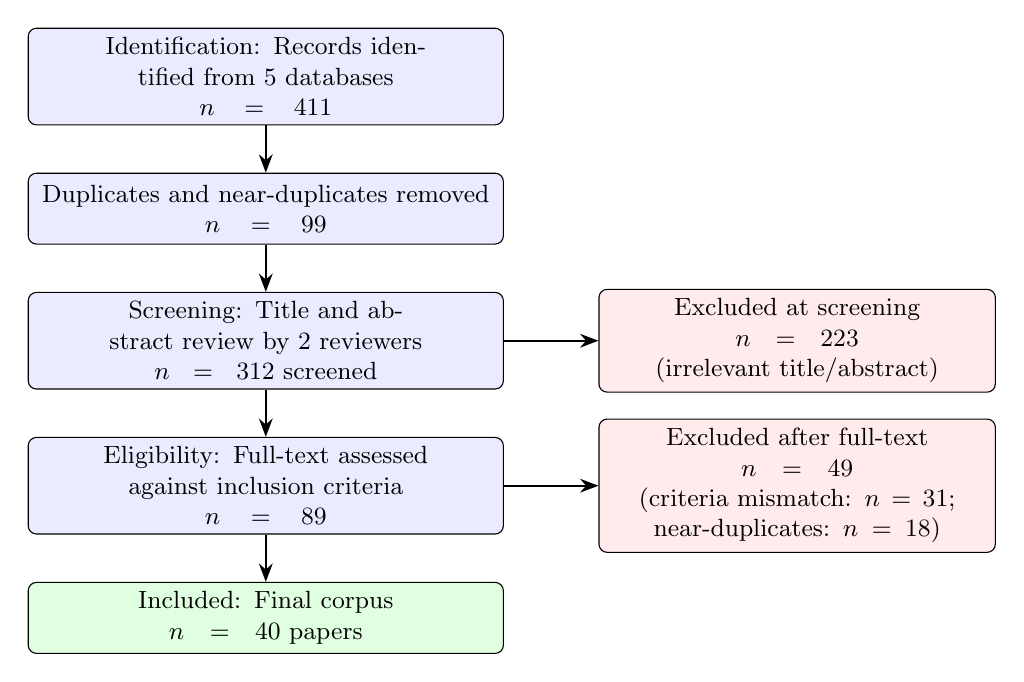
\begin{tikzpicture}[
  main/.style={rectangle, draw, rounded corners=3pt,
               text width=5.8cm, align=center,
               minimum height=0.9cm, font=\small, fill=blue!8},
  excl/.style={rectangle, draw, rounded corners=3pt,
               text width=4.8cm, align=center,
               minimum height=0.9cm, font=\small, fill=red!8},
  incl/.style={rectangle, draw, rounded corners=3pt,
               text width=5.8cm, align=center,
               minimum height=0.9cm, font=\small, fill=green!12},
  arr/.style={-{Stealth}, thick}
]
\node[main] (id)
      {Identification: Records identified from 5 databases\\$n = 411$};
\node[main, below=0.6cm of id] (dedup)
      {Duplicates and near-duplicates removed\\$n = 99$};
\node[main, below=0.6cm of dedup] (screen)
      {Screening: Title and abstract review by 2 reviewers\\$n = 312$ screened};
\node[main, below=0.6cm of screen] (elig)
      {Eligibility: Full-text assessed against inclusion criteria\\$n = 89$};
\node[incl, below=0.6cm of elig] (incl)
      {Included: Final corpus\\$n = 40$ papers};

\node[excl, right=1.2cm of screen] (exc1)
      {Excluded at screening\\$n = 223$\\(irrelevant title/abstract)};
\node[excl, right=1.2cm of elig]  (exc2)
      {Excluded after full-text\\$n = 49$\\(criteria mismatch: $n=31$;\\near-duplicates: $n=18$)};

\draw[arr] (id) -- (dedup);
\draw[arr] (dedup) -- (screen);
\draw[arr] (screen) -- (elig);
\draw[arr] (elig) -- (incl);
\draw[arr] (screen.east) -- (exc1.west);
\draw[arr] (elig.east)   -- (exc2.west);
\end{tikzpicture}
\caption{PRISMA 2020 paper selection flow for the survey corpus ($n=40$).
Of 411 records identified across five databases, 99 duplicate or
near-duplicate records were removed, leaving 312 unique records for
title/abstract screening by two independent reviewers; disagreements
were resolved by discussion or third-reviewer adjudication. Primary
exclusion reasons after full-text review: criteria mismatch ($n=31$)
and near-duplicate publications ($n=18$) that survived automated
deduplication but were caught on manual full-text inspection.}
\label{fig:prisma}
\end{figure*}

\subsection{Data Collection and Coding Process}

Each included paper was independently coded by two reviewers using a
structured coding sheet covering: (1) research lifecycle stage(s)
addressed, (2) architectural pattern(s) employed, (3) primary AI
technique, (4) evaluation method, (5) ethical/security concerns raised,
and (6) identified limitations. Where the two primary reviewers could
not reach agreement by discussion, a third reviewer adjudicated; a
fourth reviewer was consulted in the small number of cases ($n=3$)
where the third reviewer's adjudication was itself contested.
Inter-rater reliability was assessed using Cohen's $\kappa$; agreement
exceeded $\kappa = 0.78$ \cite{landis1977kappa} across all coding
dimensions before adjudication, which counts as substantial agreement.
Thematic categories were derived inductively from the coded data and
checked against the four pillars described in the Introduction.

\subsection{Quality Assessment of Included Sources}
\label{sec:quality}
The corpus mixes source types that do not share a common peer-review or validation standard: peer-reviewed journal articles, peer-reviewed conference papers, arXiv preprints, one institutional report, and several papers whose primary contribution is a prototype system or tool description rather than an empirical study. A single risk-of-bias instrument such as the Cochrane tool or ROBIS would not fit this literature; both were designed for clinical intervention studies. We instead used a lightweight, adapted checklist scored against four criteria, each rated 0–2 (absent/partial/clear): (Q1) clarity of the research question or system objective; (Q2) methodological or architectural transparency, i.e., whether the paper describes its design, pipeline, or algorithm in enough detail to assess or reproduce; (Q3) empirical validation, i.e., whether claims are backed by a reported evaluation (benchmark, user study, ablation) rather than narrative assertion alone; and (Q4) disclosure of limitations. Papers scoring 6–8 were rated \emph{High} quality, 4–5 \emph{Moderate}, 0–3 \emph{Low}. Two reviewers scored each paper independently; disagreements greater than one point on any criterion were discussed to consensus.

\begin{table}[h]
\centering
\caption{Quality-Assessment Summary by Source Type ($n=40$)}
\label{tab:quality}
\renewcommand{\arraystretch}{1.15}
\begin{tabular}{|l|c|c|c|c|}
\hline
\textbf{Source type} & \textbf{$n$} & \textbf{High} & \textbf{Moderate} & \textbf{Low} \\
\hline
Journal papers & 8 & 6 & 2 & 0 \\
\hline
Conference papers & 23 & 14 & 9 & 0 \\
\hline
Preprints (arXiv / SSRN working papers) & 6 & 2 & 4 & 0 \\
\hline
Institutional reports & 1 & 0 & 1 & 0 \\
\hline
Prototype/tool papers & 2 & 0 & 0 & 2 \\
\hline
\textbf{Total} & \textbf{40} & \textbf{22} & \textbf{16} & \textbf{2} \\
\hline
\end{tabular}
\end{table}

No paper was excluded on quality grounds alone, since the survey aims
to characterize the state of the field, including its immature and
promotional corners, rather than only its strongest evidence. Instead,
the quality rating is carried into the narrative: both papers rated
\emph{Low}, which are also the corpus's only two prototype/tool papers
reporting self-measured, non-independently-replicated performance
figures (\cite{kunekar2025omnischolar,shanmuganan2025scholargenie}),
are flagged explicitly wherever their claims are cited, and their
reported numbers are presented as self-reported rather than as
validated findings (see the critical assessments in
Section~\ref{sec:existingtools}). Appendix~\ref{app:corpus} lists the
per-paper coding and quality-assessment outcome for all 40 included
studies, so the mapping from individual paper to quality band is fully
transparent rather than aggregated only at the source-type level shown
here.


\subsection{Generative AI Use Disclosure}

While preparing this manuscript, the authors used Claude (Anthropic, Sonnet~5.5) for language editing, mainly grammar correction, sentence restructuring, and clearer phrasing. The PRISMA 2020 reporting guidelines were also consulted when structuring the systematic review methodology, including study selection, screening, and reporting.

Claude was not used to produce research data or results, to carry out the final analysis, or to draw conclusions. The authors reviewed and edited all AI-assisted text themselves and take responsibility for the accuracy and originality of the final manuscript, as required by the Taylor \& Francis Generative Artificial Intelligence (AI) Policy.

% ════════════════════════════════════════════════════════════════════════════
\section{Definitions}
\label{sec:definitions}
% ════════════════════════════════════════════════════════════════════════════

The development of research-oriented AI systems has introduced several
overlapping but distinct terms, including intelligent agents,
multi-agent systems (MAS), and agentic AI. These terms are related but
not identical; each emphasizes a different level of autonomy,
interaction, and task execution. The surveys reviewed here show a
clear shift from classical agent theory toward more flexible,
tool-using, collaborative agentic systems
\cite{falco2019mas,deshmukh2025agentic,patil2025agenticaction}.

\subsection{Intelligent Agents}
An \emph{intelligent agent} is a computational entity that exists within an environment and acts autonomously toward specific objectives. Classical definitions say it perceives its surroundings, reasons about the situation, and selects actions that move it toward its goals, so it is more than a reactive system. Falco and Robiolo associate agents with reactivity, proactivity, and social ability. The Belief-Desire-Intention (BDI) framework adds an internal cognitive structure for reasoning and action selection \cite{falco2019mas}. Such an agent should respond to changes in its environment, start actions without constant human intervention, and interact with other entities when cooperation is required.

Autonomy is central to the definition. A fully autonomous agent chooses actions from its internal state and context alone. A partially autonomous one still relies on human guidance or predefined policies. Recent work on agentic systems adds two traits: the agent adapts as new information arrives, and it communicates or coordinates with other agents or humans \cite{deshmukh2025agentic,patil2025agenticaction}. In a research workflow, this allows an agent to search for literature, summarize evidence, compare sources, and revise its output across several steps instead of in a single pass.

\subsection{Multi-Agent Systems}

A multi-agent system (MAS) is a distributed system in which several
agents share an environment and communicate with one another to solve
problems that would be difficult or impossible for a single agent to
handle alone. Agents can cooperate toward a common goal, compete for
the same resources, or mix both behaviors depending on the task. Falco
and Robiolo argue that MAS suit complex, dynamic environments because
they support interaction modeling and distributed problem solving in
ways centralized systems cannot \cite{falco2019mas}.

MAS are not only a matter of distribution; interaction matters just as
much. With multiple agents in the same system, the overall behavior
can emerge from how agents interact, not just from what each one does
on its own. That is why MAS work well for simulation, robotics,
logistics, distributed decision-making \cite{falco2019mas}, and
healthcare. The same properties that make MAS powerful also make them
hard to design and evaluate. Communication overhead, coordination
failures, inconsistent goals, and unpredictability under uncertainty
are the usual culprits.

\subsection{Agentic AI}

The term \emph{agentic AI} describes a newer generation of AI systems
that build on classical agent and MAS ideas by adding reasoning,
planning, memory, external tool use, and collaboration to autonomy.
Deshmukh et al.\ describes agentic AI as purpose-driven agents that
can break tasks into simple steps, choose actions, and adjust its strategy
over time \cite{deshmukh2025agentic}. Patil et al.\ find that recent
agentic systems increasingly rely on modular architectures,
communication layers, and coordination mechanisms, often built on
large language models (LLMs) \cite{patil2025agenticaction}.

Traditional AI and agentic AI differ in how they operate. Conventional
systems mostly handle prediction, classification, recommendation, or
generation within a fixed input-output setting. Agentic systems perform
sequences of actions, interact with external environments, and revise
their strategy as new information arrives. For research support, that
rarely means returning one response. The system runs a loop of
retrieval, cross-source evidence comparison, and judgment about how well
the available evidence supports an answer.

Recent surveys also describe agentic AI as increasingly hybrid.
Symbolic components supply reliability and interpretability, and neural
components supply flexibility and natural-language interaction
\cite{deshmukh2025agentic,patil2025agenticaction}. Research tasks need
both.

\subsection{Research AI Agents}

Research AI agents are a subclass of agentic AI built for academic and
research work. They support or automate tasks that researchers have
traditionally done by hand: literature retrieval, evidence synthesis,
citation analysis, summarization, comparative evaluation, and knowledge
discovery. Unlike conventional search engines or static recommendation
systems, they keep context across interactions and adjust their behavior
as research needs and goals change \cite{acharya2025agentic,sami2025slr}.

Recent literature increasingly treats research-oriented AI systems as
autonomous processes instead of isolated models. Sami et al.\ point out
that systematic literature reviews are slow because they require
repeated searching, filtering, screening, and synthesis of large
volumes of academic material \cite{sami2025slr}. Their proposed
multi-agent architecture gives each stage of the review to a specialized
agent: query generation, inclusion and exclusion filtering, abstraction
and summarization, and final analytical synthesis.

Because they include reasoning and memory, modern research AI agents
handle harder tasks than earlier retrieval-only systems. According to
Akuma et al., contemporary agents combine planning, memory, and
problem-solving with multi-step reasoning, external tool integration,
and task management \cite{akuma2025agents}. This lets a research agent
find information across long, unstructured texts and revise its research
questions mid-process. It can also compare sources over a long
interaction.

Distinguishing factor between research AI agents and simple retrieval systems is
how they access external resources without losing their reasoning
thread. An agent can query an academic database, identify the main
findings in matching papers, and assemble a working citation list, all
within a single continuous reasoning loop without a sequence of
prompts the user must re-enter each time
\cite{deshmukh2025agentic,acharya2025agentic}. The underlying tool
interfaces are not themselves new; databases, citation engines, and
document-management repositories have been programmatically accessible
for years. What is new is that the agent decides when to call them,
evaluates what comes back, and folds that result into its ongoing
reasoning.

Some architectures extend this with a self-reflection loop, in which
the agent compares its own output against a quality standard before
finalizing a response, and revises when the check fails
\cite{deshmukh2025agentic}. Whether this consistently produces better
results than a single well-prompted pass remains an open empirical
question, but the architecture at least makes that kind of
self-correction possible.

% ════════════════════════════════════════════════════════════════════════════
\section{Use of AI in Research}
\label{sec:useofai}
% ════════════════════════════════════════════════════════════════════════════

AI now shows up throughout research workflows, where
information volume is high, discovery moves fast, and manual
processing is not feasible. Recent work describes a shift away from
isolated task support and toward integrated systems: agents that
assist with literature discovery and evidence
synthesis, experimental planning, data analysis, scientific writing,
and even peer review.
\cite{tie2025aiscientists,kamath2025academic,gridach2025scientific}.

Table~\ref{tab:ai_research_uses} keeps two dimensions analytically
separate. \emph{Lifecycle stages} are points in the sequential,
roughly chronological path a research project follows, from topic
selection through dissemination; every stage row therefore corresponds
to a segment of \emph{when}, in a project's life, the AI capability is
used. \emph{Supporting activities} and \emph{research methods}, by
contrast, are cross-cutting: they can occur at several points in the
lifecycle (funding applications recur; qualitative-analysis tooling can
be invoked during literature review, writing, or analysis alike) and
so are not tied to a single stage. Collapsing these two dimensions into
one list, as earlier drafts of this table did, obscures which AI
capabilities are stage-bound and which are used throughout a project.

\begingroup
\renewcommand{\arraystretch}{1.25}
\scriptsize
\setlength{\tblw}{\dimexpr\textwidth-12\tabcolsep-7\arrayrulewidth\relax}
\begin{longtable}{|>{\RaggedRight\arraybackslash\hspace{0pt}}p{0.1000\tblw}|>{\RaggedRight\arraybackslash\hspace{0pt}}p{0.1433\tblw}|>{\RaggedRight\arraybackslash\hspace{0pt}}p{0.1983\tblw}|>{\RaggedRight\arraybackslash\hspace{0pt}}p{0.2117\tblw}|>{\RaggedRight\arraybackslash\hspace{0pt}}p{0.1733\tblw}|>{\RaggedRight\arraybackslash\hspace{0pt}}p{0.1733\tblw}|}
\caption{Major Uses of AI Across the Research Lifecycle, With Stages and
Cross-Cutting Support Separated}
\label{tab:ai_research_uses}\\
\hline
\textbf{Category} & \textbf{Research Stage / Activity} &
  \textbf{Representative Systems / Studies}
  & \textbf{Primary Capability} & \textbf{Main Benefit}
  & \textbf{Key Limitation} \\
\hline
\endfirsthead
\hline
\textbf{Category} & \textbf{Research Stage / Activity} &
  \textbf{Representative Systems / Studies}
  & \textbf{Primary Capability} & \textbf{Main Benefit}
  & \textbf{Key Limitation} \\
\hline
\endhead
\hline
\endfoot
\multirow{6}{=}{Lifecycle stage (sequen\-tial)} &
Stage 1: Topic exploration \& ideation &
ARC \cite{vishnumolakala2024arc} &
Topic identification, organization of early-stage work, and contextual
recommendations &
Lowers the barrier for novice researchers and supports early planning &
Limited depth without human disciplinary guidance \\
\cline{2-6}
&
Stage 2: Literature review \& knowledge extraction &
Multi-agent SLR systems \cite{sami2025slr}; Semantic Scholar, Litmaps,
Connected Papers, Research Rabbit \cite{kamath2025academic}; materials
synthesis framework \cite{lian2025literature} &
Search-string generation, screening, extraction, semantic retrieval,
and synthesis &
Cuts manual effort in large literature reviews and supports structured
evidence extraction &
Depends heavily on retrieval quality; may miss nuance in complex
sources \\
\cline{2-6}
&
Stage 3: Experimentation \& analysis &
AI4Science and agentic discovery systems
\cite{gridach2025scientific,eger2025transformingscience} &
Hypothesis generation, experiment design, and workflow orchestration &
Speeds up experimental planning and iteration &
Reproducibility and verification remain significant challenges \\
\cline{2-6}
&
Stage 4: Scientific writing &
ChatGPT-4 thesis assistant \cite{suarez2024chatgpt4}; AI Scientist
\cite{tie2025aiscientists}; AI4Research \cite{chen2025ai4research} &
Drafting, structuring, summarizing, formatting, and academic writing
support &
Speeds up drafting and gives writers more structure and confidence &
Hallucination risk, overreliance, and need for human oversight \\
\cline{2-6}
&
Stage 5: Peer review \& evaluation &
AI4Research review support \cite{chen2025ai4research}; AI Scientist
review loop \cite{tie2025aiscientists} &
Reviewer-paper matching, pre-review/meta-review drafting, and
quality-control checks &
Speeds up screening and highlights obvious issues &
Bias and verification remain significant challenges; not a substitute
for expert judgment \\
\cline{2-6}
&
Stage 6: Dissemination \& institutional governance &
Institutional AI adoption frameworks \cite{guild2024ai} &
Adoption planning, cross-disciplinary coordination, and policy
alignment for research outputs &
Gives institutions a structured path to responsible AI adoption &
Governance and infrastructure maturity vary widely by institution \\
\hline
\multirow{2}{=}{Support\-ing activity (cross-cutting)} &
Funding and proposal support &
Transdisciplinary AI tools \cite{spyroglou2021funding} &
Call-text interpretation, team matchmaking, and proposal planning &
Saves time and improves alignment with funding goals &
Strategic and institutional judgment still depend on humans \\
\cline{2-6}
&
Qualitative-research tooling and document interaction &
GPT-based qualitative workflows \cite{christou2023qualitative};
NotebookLM / ChatPDF-style interfaces \cite{eger2025transformingscience}
&
Question answering over papers, conceptualization, and thematic
analysis &
Makes academic reading and synthesis more interactive &
Fluent output can still be shallow, biased, or weakly grounded \\
\hline
\end{longtable}
\endgroup

\subsection{Research Guidance and Topic Exploration}

AI can also act as a personal research assistant. ARC, for example,
helps undergraduate engineering students identify appropriate research
topics, organize their work, and receive recommendations tailored to
their educational environment \cite{vishnumolakala2024arc}. Tools like
this matter most for students who have completed relevant coursework
but have not yet worked with an expert or research partner: their gap
is often about not knowing where to take what they already know, not
about a lack of ability.

The benefit is that AI can connect general-purpose academic tools to
the needs of an individual student. Rather than offering generic
suggestions, the system reads a student's profile and interests and
makes recommendations calibrated to their current level of
understanding \cite{vishnumolakala2024arc}.

\subsection{Literature Search, Review Automation, and Knowledge
Extraction}

Literature review automation is one of the older applications of AI in
research. Sami et al.\ show that a multi-agent system can automate most
of a literature-review pipeline: generating search strings, applying
inclusion and exclusion criteria, summarizing abstracts, and producing a
final analysis for predetermined research questions \cite{sami2025slr}.

Paper discovery and knowledge mapping are a related use. Kamath et
al.\ describe tools such as Semantic Scholar that help researchers find
relevant papers, visualize citation networks across studies, and surface
thematic links between them \cite{kamath2025academic}. Tracing citations
by hand through databases takes time, and these tools cut it down. They
can also reveal relationships that a simple keyword search would
probably miss.

AI also helps with data analysis and predictive modeling. The same
authors list environments such as Google Colab, Tableau, Power BI,
RapidMiner, Weka, H2O.ai, and Scikit-learn, which make it easier to
analyze data sets, build predictive models, and produce visualizations
\cite{kamath2025academic}. Here AI is a computational aid, not an
independent researcher. It speeds up the analysis, and the researcher
still does the interpretation.

Some systems let users converse with academic documents. Kamath et
al.\ report a generative AI application with an integrated chat feature,
built on tools such as HuggingFace and LangChain, in which users talk
directly with a PDF and ask questions about a paper instead of reading
it end to end \cite{kamath2025academic}.

Literature mining has more specialized systems. Lian et al.\ present an
automated framework for intelligent synthesis design. It filters papers
by semantic similarity, then uses progressive prompting and a
dual-agent reasoning approach to extract key experimental details from
materials-science literature \cite{lian2025literature}. The output is
structured data from papers that were never written to be
machine-readable.

\subsection{Scientific Writing, Peer Review, and Experimentation}

Some recent work covers more ambitious workflows. Tie et al.\ describe
the ``AI Scientist,'' a system designed to simulate the scientific
process end to end, from idea generation through experimentation,
writing, and paper generation \cite{tie2025aiscientists}. Their survey
finds working systems for each of these stages on its own. A fully
automated pipeline that covers all of them has not been achieved.

The scientific-discovery literature is just as broad. Gridach et al.\
report AI agents used throughout the research process: literature
review, hypothesis formulation, experimental design and execution,
scientific writing, and paper generation. The fields covered include
chemistry, biology, materials science, and engineering
\cite{gridach2025scientific}.

AI is also used for manuscript drafting and peer review. The AI4Research
survey treats scientific comprehension, academic surveying, scientific
discovery, academic writing, and peer review as interrelated processes,
not isolated tasks \cite{chen2025ai4research}. On the writing side, AI
can help draft and edit manuscript sections, improve readability,
summarize results, and format submissions to journal requirements. On
the review side, it can match papers to reviewers and handle pre-review
or meta-review tasks. Whether any of this shortens time to publication
or only moves the bottleneck is not yet clear.

Systems can extract knowledge from scientific texts and
multimodal artifacts, identify concepts, structure document content,
and give concise answers to specific questions about scientific
material \cite{chen2025ai4research}. This matters because much of what
is useful in a paper, a specific number in a table or a trend buried
in a figure, is exactly what plain-text search tends to miss.

\subsection{AI for Research Funding and Proposal Support}

Research funding preparation is now a major workload in academia:
writing proposals means interpreting call texts, aligning with
strategic policy goals, and responding to requirements on ethics,
sustainability, open science, interdisciplinarity, and impact.
Spyroglou et al.\ argue that this creates substantial pressure on
researchers and administrators, especially when success rates are low
and funding instruments are complex. They propose transdisciplinary AI
tools to support matchmaking, team composition, conceptualization, and
concretization of research plans \cite{spyroglou2021funding}.

AI can help researchers navigate the large amount of information tied
to modern calls for proposals by summarizing requirements, identifying
thematic alignment between a proposal idea and a funding call, and
cutting the time spent on document inspection. The interpretation of
funding priorities, negotiation of consortium roles, and assessment of
strategic fit still depend on researcher judgment and institutional
knowledge \cite{spyroglou2021funding}.

\subsection{Challenges and Limitations}

The same limitations keep appearing across the literature.
AI-generated content can hallucinate, lack authenticity, rest on weak
factual foundations, and be hard to replicate, especially in systems
that run several steps without human checks
\cite{gridach2025scientific,acharya2025agentic}. Ethical concerns are
just as common: transparency, citation integrity, bias, and responsible
verification. Citation integrity matters most for research. A
hallucinated citation in a paper does more damage than a hallucinated
fact in a chatbot reply.

Chubb et al.\ find that researchers see AI as useful for gathering
information and handling small tasks. They also see it as part of a
wider trend toward heavier workloads and pressure to meet academic
productivity metrics \cite{chubb2022exploring}. The same study flags
risks of bias in peer review, loss of nuance, and AI-driven research
infrastructure turning into a tool for surveillance or algorithmic
management of researchers themselves.

Qualitative-research studies raise a related caution. AI-generated
content can sound fluent but shallow, and it may contain fabricated or
misleading information \cite{christou2023qualitative}. Christou
recommends that researchers get familiar with AI output, check it for
bias, and verify it against other data sources. The analysis itself
should stay under human control, with clear evidence of the
researcher's own cognitive input throughout
\cite{christou2023qualitative}. These guidelines carry over to research
AI agents, where a human has to stay involved from the first step to the
last.

\subsection{Semantic Discovery and Document-Level Question Answering}

Recent surveys report that AI-supported literature discovery now goes
well beyond keyword matching. Researchers get something closer to a map
than a ranked list. Semantic retrieval and citation-aware exploration
let them navigate by meaning and by the relationships between papers, so
a paper can turn up even when it lacks the search terms
\cite{eger2025transformingscience}.

NotebookLM and ChatPDF-style paper-chat systems let researchers load a
small set of relevant papers and ask for targeted answers or summaries
\cite{eger2025transformingscience}. Retrieval-augmented generation
improves usability and lowers hallucination risk compared with purely
generative systems. Quality still depends on the retrieval strategy and
the grounding.

\subsection{Scientific Experimentation and Idea Generation}

AI is used for scientific idea generation and experimentation.
Eger et al.\ group this under AI4Science, which covers AI-assisted
hypothesis generation, experiment design, and automated experimentation
\cite{eger2025transformingscience}. It differs from literature
processing. That work summarizes what has been tried and this
proposes what to test next.

Hypothesis generation systems look for patterns across literature, data,
and prior experiments, then suggest candidate hypotheses
\cite{eger2025transformingscience}. They link patterns across documents
and datasets that would take much longer to assemble by hand. They 
also help with early planning by cutting a large design space down to a
few directions worth testing.

Experimentation support is more direct. AI can help with code
generation, parameter selection, and workflow orchestration, which
reduces repetitive work and shortens iteration cycles
\cite{eger2025transformingscience}.

\subsection{AI for Qualitative Research Practice}

Christou notes that AI has been used in qualitative inquiry, including
literature and systematic reviews, conceptualization, and thematic and
content analysis. These uses raise concerns about unreliability, bias,
and unethical behavior \cite{christou2023qualitative}. The concerns are
sharper than in quantitative work, because qualitative research depends
on interpretation and context, and AI systems tend to flatten both.

Christou argues that GPT-based systems can help produce summaries,
generate research questions, and support early-stage conceptualization,
but that their output should never be taken at face value
\cite{christou2023qualitative}. Qualitative research is about
interpreting meaning, not sorting content into categories. Fluent but
shallow output is therefore a particular risk, since it can pass for
analysis without doing any interpretive work.

\subsection{Institutional and Policy Perspectives on AI in Research}

The Guild's position paper on AI in research sets out the opportunities
and risks of AI in universities and research institutions, along with
the governance needed to adopt it responsibly \cite{guild2024ai}.

The report argues that AI is now widespread in academia and affects
researchers, students, educators, and administrative staff
\cite{guild2024ai}. It names literature review, hypothesis formulation,
data analysis, visualization, experimentation, and dissemination as
areas where AI can help. Alongside this, it calls for openness,
transparency, multilingual support, and cross-disciplinary collaboration.

Taken together, the literature suggests AI now plays several roles in
research: it supports research initiation through personalized
guidance, enables large-scale literature mining and structured
synthesis, automates or semi-automates systematic literature review
workflows, and shapes the broader culture of research through
productivity expectations and institutional practices
\cite{vishnumolakala2024arc,lian2025literature,bolanos2024ailitreview,chubb2022exploring}.
Systems described as hybrid, combining automation with a human-in-the-loop
checkpoint, are more often reported as working well than fully
autonomous designs (see Table~\ref{tab:comparative_evidence} for the
specific comparisons this rests on). Across sources, the recurring
theme is that AI works best when it augments human scholarship rather
than replacing it.

% ── Horizontal bar chart replacing the pie chart ───────────────────────────
\begin{figure}[ht]
\centering
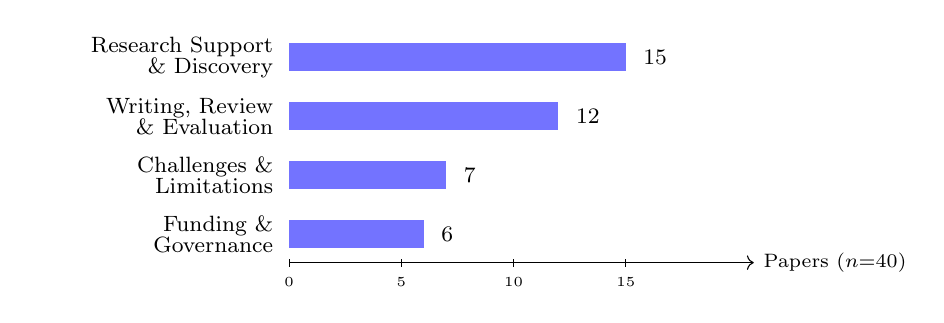
\begin{tikzpicture}[font=\footnotesize]
  % Scale: 1 paper = 0.32cm; max bar = 16*0.32 = 5.12cm
  % Left labels: ~3.5cm; right count+gap: ~0.7cm; total ~9.3cm -> use 0.28
  % 1 paper = 0.28cm; 16*0.28=4.48cm + 3.3cm label + 0.5cm count = 8.28cm OK
  \def\sc{0.285} % scale factor
  \def\bh{0.36}  % bar height cm
  \def\ys{0.75}  % vertical step between bars
  % bar 0 (bottom): Funding, 6
  \fill[blue!55] (0,0) rectangle ({6*\sc},\bh);
  \node[left, text width=3.0cm, align=right] at (-0.08,\bh/2)
        {Funding \&\\[-2pt]Governance};
  \node[right] at ({6*\sc+0.1},\bh/2) {6};
  % bar 1: Challenges, 7
  \fill[blue!55] (0,\ys) rectangle ({7*\sc},{\ys+\bh});
  \node[left, text width=3.0cm, align=right] at (-0.08,{\ys+\bh/2})
        {Challenges \&\\[-2pt]Limitations};
  \node[right] at ({7*\sc+0.1},{\ys+\bh/2}) {7};
  % bar 2: Writing, 12
  \fill[blue!55] (0,{2*\ys}) rectangle ({12*\sc},{2*\ys+\bh});
  \node[left, text width=3.0cm, align=right] at (-0.08,{2*\ys+\bh/2})
        {Writing, Review\\[-2pt]\& Evaluation};
  \node[right] at ({12*\sc+0.1},{2*\ys+\bh/2}) {12};
  % bar 3 (top): Research Support, 15
  \fill[blue!55] (0,{3*\ys}) rectangle ({15*\sc},{3*\ys+\bh});
  \node[left, text width=3.0cm, align=right] at (-0.08,{3*\ys+\bh/2})
        {Research Support\\[-2pt]\& Discovery};
  \node[right] at ({15*\sc+0.1},{3*\ys+\bh/2}) {15};
  % x-axis
  \draw[->] (0,-0.18) -- ({20*\sc+0.2},-0.18)
        node[right,font=\scriptsize] {Papers ($n{=}40$)};
  \foreach \x in {0,5,10,15}{
    \draw[thin] ({\x*\sc},-0.14) -- ({\x*\sc},-0.24)
          node[below,font=\tiny] {\x};
  }
\end{tikzpicture}
\caption{Thematic distribution of the 40 reviewed papers by primary
focus area. Counts reflect the dominant coding category per paper;
papers may address secondary themes not shown.}
\label{fig:theme-bar}
\end{figure}

As shown in Fig.~\ref{fig:theme-bar}, the reviewed corpus is dominated
by research support and discovery themes (15 papers), followed by
scientific writing, peer review, and evaluation (12 papers), while
funding/governance (6) and challenges/limitations (7) receive
comparatively less coverage.

% ════════════════════════════════════════════════════════════════════════════
\section{Architectures}
\label{sec:architectures}
% ════════════════════════════════════════════════════════════════════════════

The architecture of research AI agents sits at the intersection of
classical agent theory, large language models, retrieval pipelines,
and multi-agent orchestration. The current literature no longer
converges on a single design pattern. Instead, it points to a family
of architectural choices that differ in autonomy, coordination,
grounding, and deployment style. The Concept-Code-Commerce lens is a
useful starting point: it places AI agents across theoretical
foundations, implementation technologies, and societal deployment, and
in doing so shows that architecture must balance reasoning capability
with practical usability \cite{ishida2025conceptcodecommerce}.

An earlier version of this survey listed these architectural items,
retrieval-augmented generation, multi-agent coordination, BERT-based
evaluation models, AgentOps, and institutional integration, side by
side, as if they were mutually exclusive choices at the same level of
abstraction. They are not: they answer different questions, and a
single deployed system typically combines one item from each level.
We therefore organize the remainder of this section, and
Table~\ref{tab:architecture_comparison}, around four taxonomic levels:

\begin{itemize}
  \item \textbf{Level 1 -- Component techniques.} Building blocks used
  \emph{inside} an agent to perform a specific function: retrieval-augmented
  generation (Section~\ref{sec:rag}) for grounding, and
  task-specific fine-tuned models such as BERT-based evaluators
  (Section~\ref{sec:classicalllm}) for scoring or classification. A
  component technique is not itself a complete agent.
  \item \textbf{Level 2 -- Agent architecture patterns.} How an
  individual agent, or a coordinated set of agents, is structured and
  makes decisions: classical agent models, LLM-based agents, Agentic
  RAG, Multi-Agent Autonomous Workflow Systems (MAWS), TacTool-style
  tool-calling separation, and closed-loop autonomous-discovery
  architectures (Sections~\ref{sec:classicalllm}--\ref{sec:tactool}).
  This is the level most prior surveys treat as the only level.
  \item \textbf{Level 3 -- Operational management layer.} Cross-cutting
  infrastructure for running and maintaining an agent \emph{regardless
  of which Level-2 pattern it uses}: AgentOps-style observability,
  monitoring, and automated tuning (Section~\ref{sec:tactool}).
  \item \textbf{Level 4 -- Deployment and institutional integration.}
  How an agent architecture is adopted at organizational scale:
  enterprise governance layers and library/institutional integration
  frameworks (Section~\ref{sec:enterprise}). This level is about
  organizational readiness and governance, not about how the agent
  itself reasons.
\end{itemize}

Table~\ref{tab:architecture_comparison} makes this level assignment
explicit for all twelve architecture-related items identified in the
corpus, which keeps the comparison honest: it no longer implies, for
example, that RAG (a Level-1 technique) and enterprise governance (a
Level-4 deployment concern) compete for the same design decision.

\subsection{Classical Foundations and LLM-Based Agent Architectures}
\label{sec:classicalllm}

Early architectural ideas in AI agents centered on autonomy,
decision-making, and coordination. Ishida et al.\ trace these ideas to
foundational work on the Blackboard Model and the Contract Net
Protocol, which established early mechanisms for distributed problem
solving and negotiated task allocation among agents
\cite{ishida2025conceptcodecommerce}. The main classical families
within autonomous agent research are reactive, deliberative, layered,
and learning-based models.

Large language models have reshaped agent architecture by adding
natural language reasoning, instruction following, and tool
orchestration to the traditional autonomy stack. Chen and Peng
describe an LLM-based AI agent as a system built around four core
components: the LLM itself, a memory module, task-planning capability,
and a tool-usage mechanism \cite{chen2025llmagent}. Separating
language understanding from state retention, planning, and external
action makes this architecture useful.

Prompt engineering is a central design element in these
architectures. Chen and Peng argue that prompts form the control layer connecting user intent to the
agent's reasoning process \cite{chen2025llmagent}. In practice, the
most workable LLM-based architecture is a modular system where memory, planning,
tools, and reasoning are handled separately
\cite{chen2025llmagent,ishida2025conceptcodecommerce}.

\subsection{Retrieval-Augmented Architectures (Level 1: Component Technique)}
\label{sec:rag}

Retrieval-augmented generation is a common architecture for
research-oriented agents as it pairs language generation with
grounding in external sources. Han et al.\ describe RAG as a
three-stage pipeline: retrieval, augmentation, and generation
\cite{han2024ragslr}. This reduces reliance on static pretraining and
limits hallucination when a research problem needs up-to-date or
source-backed answers.

This architecture matters for systematic literature review
automation. Han et al.\ propose an RAG-based framework covering four
core SLR stages: literature search, literature screening, data
extraction, and information synthesis \cite{han2024ragslr}. RAG makes
the research agent more verifiable as the agent can point to retrieved
scientific sources.

Sparse retrievers such as BM25 are efficient and interpretable, but
they lean heavily on keyword overlap. Dense retrievers capture
semantic similarity and handle nuanced academic queries better, though
they cost more to run. Search engines can also work as retrievers when
the system needs current information \cite{han2024ragslr}.

\subsection{Multi-Agent Autonomous Workflow Architectures (Level 2: Agent Pattern)}
\label{sec:maws}

A second architectural pattern uses multiple autonomous agents that work
together through explicit workflows. Apuri and Yepuri define Multi-Agent
Autonomous Workflow Systems (MAWS) as systems in which autonomous agents
collaborate, reassign tasks dynamically, and adapt to changing conditions
in their environment \cite{apuri2026maws}. Centralized workflow
management is rigid. MAWS distributes authority instead, and the agents
coordinate around shared objectives without a fixed central schedule.

A distinguishing feature of MAWS is agent specialization and the
communication links between agents. Each agent can make independent
decisions based on the information it receives, inform other agents,
and adjust its behavior in response to environmental conditions
\cite{apuri2026maws}. The paper also reports using methods such as
deep reinforcement learning and collaborative multi-agent learning to
improve policy choice and coordination, alongside collaborative
planning and hierarchical task organization as further architectural
patterns.

\subsection{Agentic RAG: From Traditional RAG to Adaptive Pipelines (Level 2: Agent Pattern)}
\label{sec:agenticrag}

Agentic RAG is an answer to the limits of
standard retrieval-augmented generation \cite{singh2025agentrag}.
Traditional RAG systems follow a largely linear, static path. Agentic
RAG adds decision-making around the retrieve-augment-generate cycle,
so the pipeline can adjust as it runs.

Singh et al.\ identify four core agent components that make this
possible: the LLM, memory, planning, and tools. Together these make
the agent stateful and adaptive rather than stateless and reactive
\cite{singh2025agentrag}. They also identify four recurring agentic
workflow patterns, reflection, planning, tool use, and multi-agent
collaboration, implemented through common workflow structures such as
prompt chaining, routing, parallelization, orchestrator-worker
systems, and evaluator-optimizer designs.

The taxonomy starts with the single-agent architecture, where one
coordinating agent handles query analysis, source selection,
retrieval, and response synthesis. The multi-agent extension separates
coordination from retrieval and synthesis: a master retrieval agent
delegates to specialized agents \cite{singh2025agentrag}. Graph RAG
adds graph structures to represent relationships among entities,
concepts, and documents, which enables multi-hop reasoning and
contextual enrichment.

\begin{figure}[ht]
\centering
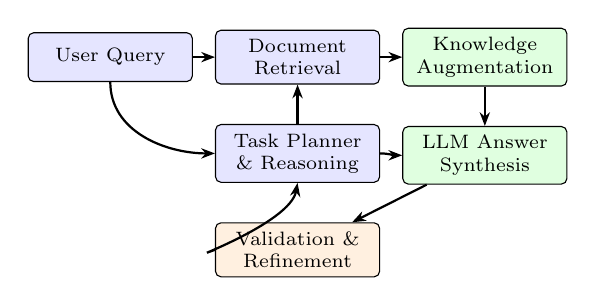
\begin{tikzpicture}[
  node distance=0.38cm and 0.28cm,
  box/.style={rectangle, draw, rounded corners=2pt,
    text width=1.85cm, align=center,
    minimum height=0.62cm, font=\scriptsize},
  sbox/.style={box, fill=blue!10},
  dbox/.style={box, fill=green!12},
  vbox/.style={box, fill=orange!12},
  arr/.style={-{Stealth[scale=0.75]}, thick}
]
\node[sbox] (q)    {User Query};
\node[sbox, right=0.28cm of q]  (ret)  {Document Retrieval};
\node[dbox, right=0.28cm of ret](aug)  {Knowledge Augmentation};
\node[sbox, below=0.50cm of ret](plan) {Task Planner \& Reasoning};
\node[dbox, below=0.50cm of aug](llm)  {LLM Answer Synthesis};
\node[vbox, below=0.50cm of plan](val) {Validation \& Refinement};
\draw[arr](q)--(ret);
\draw[arr](ret)--(aug);
\draw[arr](aug)--(llm);
\draw[arr](q.south) to[out=270,in=180] (plan.west);
\draw[arr](plan)--(ret);
\draw[arr](plan.east) to[out=0,in=180] (llm.west);
\draw[arr](llm)--(val);
\draw[arr](val.west) to[out=200,in=260] (plan.south);
\end{tikzpicture}
\caption{Agentic RAG pipeline for systematic literature review. Adapted
from~\cite{singh2025agentrag}. The system extends traditional RAG with
iterative feedback loops, multi-step reasoning, and adaptive retrieval,
enabling context-aware knowledge synthesis and validation.}
\label{fig:agentic_rag}
\end{figure}

\subsection{Tactical Tool-Calling (Level 2) and AgentOps (Level 3)}
\label{sec:tactool}

Reliable tool usage is a central challenge in agentic AI architecture.
Singh et al.\ note that even strong models can fail at
reasoning about whether a tool is needed or they fail at formatting the call
itself \cite{singh2025tactool}. TacTool separates these two problems:
one LLM reasons and produces a concise plan, while a second LLM calls
the tool and executes the function. A response-selection layer then
compares the two outputs using an LLM-as-a-judge mechanism, so the
system can recover from partial failures \cite{singh2025tactool}.
TacTool is a Level-2 agent pattern: it changes how a single agent
decides to act.

AgentOps, by contrast, sits at Level 3: it does not change how an
agent reasons. It wraps around whichever Level-2 pattern is deployed
to keep it observable and maintainable at runtime. Autonomy brings
operational uncertainty. Moshkovich and Zeltyn
argue that agentic systems are inherently probabilistic: they depend
on LLM reasoning, changing memory states, shifting tool availability,
and execution paths that evolve at runtime
\cite{moshkovich2025agentops}. Their AgentOps framework runs as a
six-stage pipeline: observe behavior, collect metrics, detect issues,
identify root causes, generate recommendations, and automate
operations.

\begin{figure*}[t]
\centering
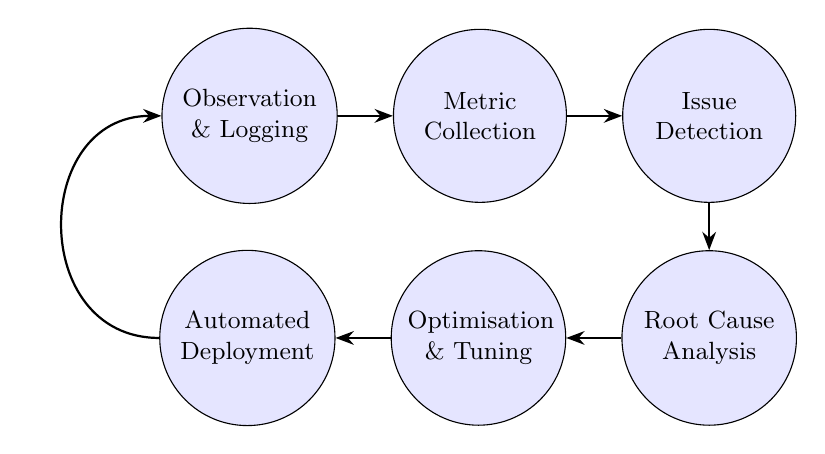
\begin{tikzpicture}[
  every node/.style={font=\small},
  circ/.style={circle, draw, fill=blue!10,
    text width=1.8cm, align=center, minimum size=1.8cm},
  arr/.style={-{Stealth},thick}
]
\node[circ] (obs)  {Observation \& Logging};
\node[circ, right=0.7cm of obs]  (met) {Metric Collection};
\node[circ, right=0.7cm of met]  (iss) {Issue Detection};
\node[circ, below=0.6cm of iss]  (rca) {Root Cause Analysis};
\node[circ, left=0.7cm  of rca]  (opt) {Optimisation \& Tuning};
\node[circ, left=0.7cm  of opt]  (dep) {Automated Deployment};
\draw[arr](obs)--(met); \draw[arr](met)--(iss);
\draw[arr](iss)--(rca); \draw[arr](rca)--(opt);
\draw[arr](opt)--(dep);
\draw[arr](dep.west) to[out=180,in=180,looseness=1.5] (obs.west);
\end{tikzpicture}
\caption{AgentOps lifecycle for managing uncertainty in agentic AI
systems. Adapted from~\cite{moshkovich2025agentops}. The pipeline forms
a continuous feedback loop for system reliability and adaptation.}
\label{fig:agentops}
\end{figure*}

\subsection{Autonomous Scientific Discovery and Layered NLP Architectures (Level 2), and BERT-Based Evaluation (Level 1)}
\label{sec:autonomous}

Kohli et al.\ describe autonomous AI agents as systems capable of
planning, learning, experimentation, reasoning, and adaptation inside
closed-loop scientific workflows \cite{kohli2025autonomous}. They
identify five coupled capabilities underlying this architecture:
perception, planning and reasoning, learning, execution, and
adaptation. One concept that follows from this work is the
``self-driving laboratory,'' where AI planning systems connect
directly to robotic experimental infrastructure. Closed-loop systems
of this kind raise open questions about reproducibility,
interpretability, trust, and safety \cite{kohli2025autonomous}. Like
MAWS and Agentic RAG, this is a Level-2 agent pattern.

Sharma et al.\ report that, on their text-classification benchmark,
an agentic architecture combining adaptive learning, memory retrieval,
multi-agent collaboration, and reinforcement-based refinement
outperformed the static classifiers they compared it against
\cite{sharma2025textclassification}; this is a study-specific,
single-paper comparison rather than a corpus-wide finding. Their
architecture has five layers: Perception, Memory and Knowledge Base,
Decision Engine, Actuation, and Feedback and Learning, again a Level-2
pattern. Chen takes a narrower approach and proposes a BERT-centered model for
academic writing evaluation. The model splits assessment into
preprocessing, contextual embedding, specialized classifiers, holistic
scoring, and feedback generation \cite{chen2025emiwriting}. This is a
Level-1 component technique. It is a fine-tuned scoring model that could
sit inside a larger agent, but it is not an agent architecture itself.
We therefore treat it separately from the Level-2 pattern of Sharma et
al., although both papers use the word ``architecture.''

\subsection{Enterprise-Scale and Library Integration Architectures (Level 4: Deployment)}
\label{sec:enterprise}

According to Singh et al., agentic workflows add autonomous cycles of
refinement, planning, and collaboration before the final response is
produced \cite{singh2024agenticworkflows}. The common patterns are
reflection, tool use, planning, and multi-agent collaboration. Pandey
and Narnag build on this with the Integrated Agentic Foundry (IAF), a
governance-first architecture with four layers: foundational
(multimodal knowledge graph), cognitive orchestration, embodied
perception-and-action, and governance-and-interoperability
\cite{pandey2025agenticenterprise}. The governance layer adds
standardized protocols such as Model Context Protocol (MCP) and
Agent-to-Agent (A2A) communication.

Ivanova's engineering framework covers the integration of AI into
research and academic library infrastructures \cite{ivanova2025libraryai}.
It divides adoption into three stages: organizational preparation,
implementation of AI-ready solutions, and integration of external AI
expertise. The paper cites UNESCO's ethical standards and the European
Union AI Act as guidance.

\subsection{Architectural Trade-Offs and Comparative Analysis}

Full comparison in Supplementary Table~\ref{tab:architecture_comparison}.

Table~\ref{tab:architecture_comparison} summarizes the twelve
architecture-related items reviewed, now organized by the four
taxonomic levels introduced above rather than listed as a single flat
inventory. No single Level-2 pattern is universally optimal.
Lightweight LLM agents are flexible but may lack grounding.
RAG systems improve factual reliability but depend heavily on retrieval
quality. Multi-agent systems increase scalability but introduce
coordination overhead. Enterprise-scale and institutional architectures
provide governance and interoperability but require substantial
infrastructure \cite{pandey2025agenticenterprise,ivanova2025libraryai}.

For research AI agents specifically, hybrid modular architectures,
those combining LLM reasoning, retrieval grounding, memory systems,
tool orchestration, and observability mechanisms into one coordinated
framework, are more frequently reported as outperforming monolithic or
single-technique designs. Table~\ref{tab:comparative_evidence}
collects the specific within-paper comparisons this claim rests on. We
are explicit about what this evidence does and does not show: each row
is a comparison reported \emph{within one primary study}, typically
against a baseline the same authors defined, not a controlled,
head-to-head benchmark run across architectures by an independent
third party. No paper in the corpus benchmarks two or more of these
architecture families against each other under identical tasks and
metrics. The pattern is therefore best read as a convergent signal
across independent research teams rather than as settled comparative
proof, which is why we phrase it as a frequently-reported finding
rather than a validated result.

\begin{table}[h]
\centering
\caption{Within-Study Comparative Evidence Cited for the Hybrid-Modular
Pattern}
\label{tab:comparative_evidence}
\renewcommand{\arraystretch}{1.25}
\begin{tabularx}{\columnwidth}{|>{\RaggedRight\arraybackslash}p{0.14\columnwidth}|>{\RaggedRight\arraybackslash}X|>{\RaggedRight\arraybackslash}p{0.30\columnwidth}|}
\hline
\textbf{Source} & \textbf{Comparison reported} & \textbf{Nature of evidence} \\
\hline
\cite{sharma2025textclassification} &
Layered agentic architecture (perception, memory, decision, actuation,
feedback) outperformed static classifiers on the authors' own
text-classification benchmark &
Single-paper benchmark, author-defined baseline \\
\hline
\cite{singh2025tactool} &
Two-LLM TacTool design (separate reasoning and execution roles) reduced
malformed tool calls relative to a single-LLM tool-calling baseline &
Single-paper ablation, author-reported \\
\hline
\cite{han2024ragslr} &
RAG pipelines reduced unsupported/hallucinated claims relative to
generation without retrieval grounding, across the SLR studies
surveyed &
Narrative synthesis across multiple primary studies, not a new
head-to-head experiment \\
\hline
\cite{kunekar2025omnischolar} &
Multi-agent CrewAI pipeline reported higher accuracy and lower
processing time than the authors' own non-agentic baseline pipeline &
Single-paper, self-reported; rated \emph{Low} quality
(Section~\ref{sec:quality}) -- included here for completeness, not as
independent corroboration \\
\hline
\end{tabularx}
\end{table}

\begin{table*}[t]
\centering
\caption{Architectural Statistics Extracted from the Reviewed Literature}
\label{tab:architecture_stats}
\begin{tabularx}{\linewidth}{@{}l c X@{}}
\toprule
\textbf{Architectural Element} & \textbf{Count} & \textbf{Description}
\\
\midrule
Classical agent families & 4 &
Reactive, deliberative, layered, and learning-based architectures. \\
Core LLM-agent components & 4 &
LLM, memory, planning, and tool-usage modules. \\
RAG pipeline stages & 3 &
Retrieval, augmentation, and generation. \\
SLR workflow stages & 4 &
Literature search, screening, data extraction, and synthesis. \\
Agentic workflow patterns & 4 &
Reflection, planning, tool use, and multi-agent collaboration. \\
AgentOps operational stages & 6 &
Observation, metric collection, issue detection, root-cause analysis,
optimization, and automation. \\
Layered text-classification modules & 5 &
Perception, memory, decision engine, actuation, and feedback-learning
layers. \\
\bottomrule
\end{tabularx}
\end{table*}

\begin{figure*}[t]
\centering
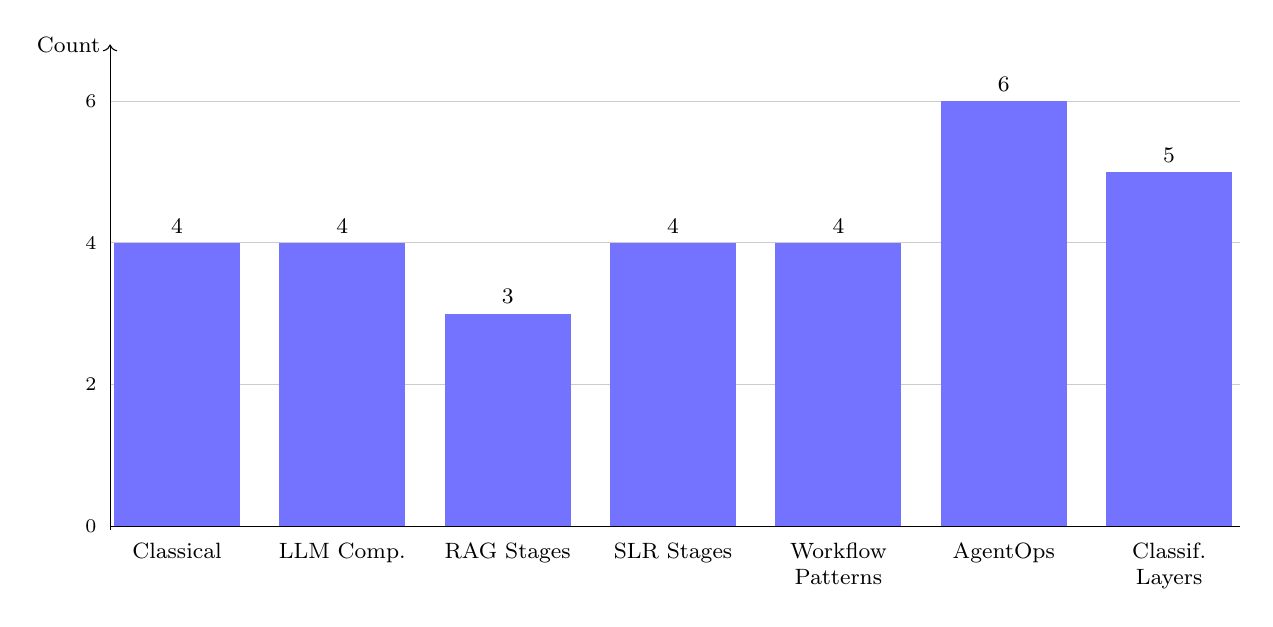
\begin{tikzpicture}[x=1cm, y=0.9cm, font=\small]
  % Bar width=1.6cm, gap=0.5cm, y-unit=0.9cm
  % 7 bars total width = 7*1.6+6*0.5 = 14.2cm -- fits textwidth
  \def\bw{1.6}
  \def\bg{0.5}
  % Draw gridlines
  \foreach \y in {0,2,4,6} {
    \draw[thin,gray!40] (-0.05,\y) -- ({6*(\bw+\bg)+\bw+0.1},\y);
    \node[left,font=\scriptsize] at (-0.1,\y) {\y};
  }
  % y-axis
  \draw[->] (-0.05,-0.05) -- (-0.05,6.8) node[left,font=\footnotesize] {Count};
  % x-axis baseline
  \draw (-0.05,0) -- ({6*(\bw+\bg)+\bw+0.1},0);
  % Bars and labels
  \foreach \val/\lbl [count=\i from 0] in
    {4/Classical, 4/{LLM Comp.}, 3/{RAG Stages}, 4/{SLR Stages},
     4/{Workflow Patterns}, 6/AgentOps, 5/{Classif. Layers}} {
    \pgfmathsetmacro{\xl}{\i*(\bw+\bg)}
    \pgfmathsetmacro{\xr}{\i*(\bw+\bg)+\bw}
    \pgfmathsetmacro{\xm}{\i*(\bw+\bg)+\bw/2}
    \fill[blue!55] (\xl,0) rectangle (\xr,\val);
    \node[above,font=\footnotesize] at (\xm,\val) {\val};
    \node[below,text width=1.7cm,align=center,font=\footnotesize]
          at (\xm,-0.1) {\lbl};
  }
\end{tikzpicture}
\caption{Architectural patterns and workflow structures identified in the
reviewed AI-agent literature. Surveyed systems consistently emphasise
modular architectures, retrieval grounding, planning, multi-agent
coordination, and operational observability for literature-review
automation.}
\label{fig:architecture_stats}
\end{figure*}

% ════════════════════════════════════════════════════════════════════════════
\section{The Proposed Architectural-Lifecycle Framework}
\label{sec:framework}
% ════════════════════════════════════════════════════════════════════════════

The abstract of this survey claims an original architectural and
lifecycle-based framework. We make that framework explicit here rather
than leaving it implicit in the preceding two sections, and we state
directly how it differs from the three closest prior surveys.

\subsection{Structure of the Framework}

The framework has two axes, developed independently in
Section~\ref{sec:useofai} (the six-stage lifecycle,
Table~\ref{tab:ai_research_uses}) and Section~\ref{sec:architectures}
(the four-level architectural taxonomy, Table~\ref{tab:architecture_comparison}).
Its contribution is to cross them: for each lifecycle stage, it
identifies which architectural level currently carries the AI
capability used at that stage, and which levels are absent. This
answers a question neither axis answers alone: not just ``what does AI
do at this stage'' (the lifecycle table) and not just ``how is an
agent built'' (the architecture table), but ``which class of
architecture is actually responsible for supporting this stage today,
and is that support structurally adequate or merely incidental.''

Each stage$\times$level cell in Table~\ref{tab:framework} is rated
against one criterion: \emph{how many of the reviewed papers report a
system at that level explicitly targeting that lifecycle stage, and
how developed is that reported system}. We apply this consistently
using four bands: \emph{Absent} means no paper in the corpus reports a
system at that level for that stage; \emph{Weak} means one paper
reports a system, but it is a narrow or repurposed use (e.g., a
general-purpose LLM agent applied to the stage without a
stage-specific design) rather than a purpose-built pattern; \emph{Partial}
means two or more papers report systems, but they are early-stage,
evaluated only informally, or address only part of the stage's tasks;
\emph{Strong} means three or more papers report systems that are
purpose-built for the stage and include at least some reported
evaluation (benchmark, case study, or user study, per the Q3 criterion
in Section~\ref{sec:quality}). The same two reviewers who conducted
the coding in Section~\ref{sec:methodology} assigned these bands
independently, using the coding sheet's lifecycle-stage and
architectural-pattern fields, and resolved disagreements by discussion.

\begingroup
\renewcommand{\arraystretch}{1.25}
\scriptsize
\setlength{\tblw}{\dimexpr\textwidth-12\tabcolsep-7\arrayrulewidth\relax}
\begin{longtable}{|>{\RaggedRight\arraybackslash\hspace{0pt}}p{0.1967\tblw}|>{\RaggedRight\arraybackslash\hspace{0pt}}p{0.1550\tblw}|>{\RaggedRight\arraybackslash\hspace{0pt}}p{0.1550\tblw}|>{\RaggedRight\arraybackslash\hspace{0pt}}p{0.1550\tblw}|>{\RaggedRight\arraybackslash\hspace{0pt}}p{0.1550\tblw}|>{\RaggedRight\arraybackslash\hspace{0pt}}p{0.1833\tblw}|}
\caption{The Architectural-Lifecycle Framework: Cross-Mapping of Lifecycle
Stage Against Architectural Level}
\label{tab:framework}\\
\hline
\textbf{Lifecycle Stage} & \textbf{L1: Technique present}
  & \textbf{L2: Agent pattern present} & \textbf{L3: Operational layer
  present} & \textbf{L4: Deployment layer present}
  & \textbf{Structural gap} \\
\hline
\endfirsthead
\hline
\textbf{Lifecycle Stage} & \textbf{L1: Technique present}
  & \textbf{L2: Agent pattern present} & \textbf{L3: Operational layer
  present} & \textbf{L4: Deployment layer present}
  & \textbf{Structural gap} \\
\hline
\endhead
\hline
\endfoot
1. Topic exploration \& ideation &
Weak (profile-based recommendation only) &
No dedicated pattern; single-turn LLM use &
Absent &
Absent &
No agent architecture yet targets this stage specifically \\
\hline
2. Literature review \& knowledge extraction &
Strong (RAG is the default grounding technique) &
Strong (Agentic RAG, MAWS, multi-agent SLR systems) &
Partial (AgentOps applies but is rarely reported \emph{for} this
stage) &
Weak &
Best-covered stage overall; operational monitoring is the main gap \\
\hline
3. Experimentation \& analysis &
Weak (task-specific models, not yet standardized) &
Partial (autonomous-discovery patterns exist but are early-stage) &
Absent &
Absent &
Closed-loop safety and reproducibility controls are largely
undeveloped \\
\hline
4. Scientific writing &
Partial (BERT-based evaluators for scoring) &
Partial (LLM-based agent pattern, not writing-specific) &
Absent &
Absent &
No writing-specific agent pattern; relies on general LLM agents \\
\hline
5. Peer review \& evaluation &
Weak &
Weak (folded into AI4Research as a task, not a dedicated pattern) &
Absent &
Absent &
Least architecturally developed stage in the corpus \\
\hline
6. Dissemination \& institutional governance &
Absent &
Absent &
Absent &
Strong (Enterprise Agentic, Library AI Integration) &
Governance frameworks exist but are decoupled from the agent patterns
used earlier in the pipeline \\
\hline
\end{longtable}
\endgroup

\subsection{What the Framework Shows}

Two patterns stand out. First, architectural maturity is concentrated
at Stage 2 (literature review) and, separately, at Level 4
(institutional deployment); these two areas of strength do not overlap
with each other, since the enterprise and library-integration
architectures reviewed in Section~\ref{sec:enterprise} are described
at the organizational level and are not reported as wrapping the
literature-review agent patterns reviewed in
Section~\ref{sec:agenticrag}. Second, Stages 1, 3, and 5 (ideation,
experimentation, and peer review) each lack a dedicated Level-2 agent
pattern: the AI capability used there is either a general-purpose LLM
agent repurposed for the task, or, in the case of experimentation, an
early-stage closed-loop system whose safety and reproducibility
properties are still open questions \cite{kohli2025autonomous}. No
paper in the corpus proposes an AgentOps-style operational layer
(Level 3) for any stage other than literature review, which means
runtime monitoring, once a system is deployed for writing support,
experimentation, or peer review, is largely unaddressed by the
reviewed literature.

\subsection{Differentiation From Prior Surveys}

This cross-mapping is what distinguishes the present framework from
the three closest prior surveys, extending the comparison introduced
in Section~\ref{sec:introduction}. Bola\~nos et al.\
\cite{bolanos2024ailitreview} analyze architectural choices only
within Stage 2 and do not extend the comparison to other lifecycle
stages or to Levels 3--4. Gridach et al.\ \cite{gridach2025scientific}
survey agentic techniques across several stages but do not organize
those techniques into the leveled taxonomy used here, so their survey
cannot distinguish, for example, a Level-1 technique from a Level-4
deployment concern. Chen et al.\ \cite{chen2025ai4research} catalog
AI4Research tasks stage-by-stage but treat architecture as incidental
detail rather than as a second, independently structured axis. None of
the three produces a table analogous to
Table~\ref{tab:framework} that lets a reader see, at a glance, which
lifecycle stages are architecturally underserved.

% ════════════════════════════════════════════════════════════════════════════
\section{Existing Tools}
\label{sec:existingtools}
% ════════════════════════════════════════════════════════════════════════════

\subsection{General-Purpose LLM Assistants}

\subsubsection{ChatGPT-4 for Thesis Development}

In the case study reviewed, ChatGPT-4 was tested as an academic
assistant for postgraduate thesis development, supporting definition
of the research problem, the literature review, and formulation of
the research hypothesis \cite{suarez2024chatgpt4}.

NotebookLM is a retrieval-based note-taking tool, developed by Google
Labs (built on Google's Gemini models) rather than by Google DeepMind,
where users upload their own source documents instead of
searching the open web and query directly against their own
notebooks.\footnote{Verified against Google's own product
documentation at \url{https://notebooklm.google} as of September 2026;
an earlier draft of this survey misattributed development to Google
DeepMind.} Hallucination risk is reduced by this closed-corpus Q\&A
design, since answers are bound to the uploaded content rather than
to a general chat interface. Eger et al.\ categorize NotebookLM under
a broader umbrella of paper-chat tools designed for focused academic
reading \cite{eger2025transformingscience}. The downside is that the
tool's scope is limited to what the user uploads, so it is not
well-suited to a thorough literature review on its own.

Elicit is an AI research assistant that automates part of the
literature review. It searches for papers, pulls out their key claims,
and fills in structured comparison tables. The user poses a research
question, and Elicit returns a ranked list of papers with the
methodology, findings, and limitations of each. The
output fields and extraction templates are built to align with
systematic-review conventions. Elicit's own documentation describes its
corpus as built primarily on the Semantic Scholar dataset rather than
as a single-source index; even so, coverage is uneven across
disciplines (weighted toward biomedical and social-science literature),
and extraction quality drops for specialized or interdisciplinary
topics that the underlying corpus covers less well. Coverage claims for
commercial tools such as Elicit change without notice and should be
re-verified against the vendor's current documentation before
publication.

\subsubsection{Consensus} Consensus is a search engine for scientific papers that can produce a consensus based on evidence rather than keyword matching at the study level. It pulls apart relevant papers and generates a consensus meter that rates the support or rejection of a specific claim in the literature, useful for evidence-checking or to support a hypothesis before further digging. There's one big problem with the meter, however: it collapses all the research, irrespective of design and sample size, and fails to account for the quality of the research; as a result, it can give the impression of a more stable or definitive summary than the actual study results.

\subsection{Literature Discovery Platforms}

\subsubsection{Semantic Scholar} Semantic Scholar, from the Allen Institute for AI, is a large-scale academic search engine built on NLP-based semantic indexing and citation analysis. It handles semantic search, paper recommendations, citation graph navigation, and TLDRs, one-sentence summaries of each paper. Kamath et al.\ describe it as useful for mapping knowledge and spotting thematic relationships between papers \cite{kamath2025academic}. It also quietly does a lot of heavy lifting behind the scenes: several multi-agent tools, including OmniScholar and ScholarGenie, use it as their retrieval backbone. Semantic Scholar itself does not support interactive synthesis or structured extraction natively.

\subsubsection{Connected Papers} Connected Papers builds a visual citation network around a seed paper, letting researchers navigate related work through graph visualization instead of keyword search. Each node is a paper, each edge a citation relationship, and node size tracks citation count. Kamath et al.\ note its value for surfacing thematically related papers that might not share a single keyword with the seed \cite{kamath2025academic}. The tool earns its keep in the exploratory phase of a literature review, but that's where it stops: no extraction, no summarization, no synthesis.
\subsubsection{Research Rabbit} Research Rabbit is a free citation-graph tool that turns a seed set of papers into an interactive map of related literature. What sets it apart from Connected Papers is that the network isn't fixed. Users can keep refining it, adding papers, dropping ones that turn out to be dead ends, and the tool also plugs into Zotero for reference management. The downside shows up at scale: feed it a large seed set and the graph gets tangled fast, and there is no automated summarization to fall back on.
\subsubsection{Litmaps} Litmaps generates chronological citation maps of how a research area has developed: when the key papers appeared, how later work cited them, and where gaps remain. Kamath et al.\ describe it as a tool for detecting thematic relationships across studies \cite{kamath2025academic}. It tracks research trajectories and points out influential work, but it stops there. The researcher still does the extraction and synthesis.
\subsubsection{Scite.ai} Scite.ai labels citations as supporting, contradicting, or merely mentioning a claim, which says more than a raw citation count. Researchers can use these ``smart citation'' labels to see whether a finding has been replicated or challenged, or only cited in passing. Systematic reviewers can use them to judge how much weight a claim can bear. Accuracy varies by domain, and coverage is thinner for older and non-English literature.

\subsection{Multi-Agent Synthesis Systems}

\subsubsection{OmniScholar for Researcher Profiling and SDG Mapping}

OmniScholar is a tool for automatically extracting, structuring, and
interpreting the bibliographic metadata of a researcher's publications
\cite{kunekar2025omnischolar}. Google Scholar, ResearchGate, and
Semantic Scholar are all large stores of publication data, but none of
them automate the full process of profiling an author, filtering their
work, and correlating it to thematic objectives such as the UN
Sustainable Development Goals (SDGs); that is the gap OmniScholar is
designed to fill.

The authors compare two architectures head to head: a multi-agent
CrewAI pipeline, with separate agents for retrieval, Gemini-based
formatting, and TF-IDF SDG mapping, versus a non-agentic pipeline that
queries Semantic Scholar, CrossRef, and other sources directly through
a custom API process \cite{kunekar2025omnischolar}. The highest
accuracy reported was 92\% for keyword-based SDG classification, and a
ranking system integrates citation counts, publication dates, author
relevance, and SDG similarity into a single composite score. The paper
also reports a time saving of more than 95\% relative to manual
profiling.

\paragraph{Critical Assessment.} As flagged in the quality assessment
(Section~\ref{sec:quality}, Table~\ref{tab:quality}), this paper is
rated \emph{Low} quality: the numbers come from a single conference
paper with no independent evaluation or adversarial testing. The 92\%
accuracy figure is measured against a dataset the authors themselves
constructed, and the 95\% time-reduction figure is not accompanied by
any described control condition. The scraping component is also
fragile: a change to a source website's structure, or an ambiguous
author name, can break it. The output is interesting but unbenchmarked
and should be treated as indicative rather than validated; we
recommend manual verification of OmniScholar's output before using it
for institutional reporting.

\subsubsection{ScholarGenie for Automated Literature Summarization and Presentation Generation}

ScholarGenie is a modular multi-agent framework built on CrewAI and
LangChain. A single pipeline covers literature retrieval, semantic
summarization, and slide generation \cite{shanmuganan2025scholargenie}.
It consists of an Autonomous Literature Agent, a Semantic Contextual
Summarizer, a GenieSlide Generator, and an optional text-to-speech
agent. Before anything reaches the summarizer, retrieval goes through
topic expansion, synonym rewriting, and relevance ranking. The
summarizer then splits each paper into problem statement, methodology,
key findings, and limitations. The paper reports that literature
processing takes up to 80\% less time and that slide decks are
generated in under a minute.

\paragraph{Critical Assessment.} ScholarGenie has the same weakness as
OmniScholar and receives the same \emph{Low} quality rating
(Table~\ref{tab:quality}). Its results come from a single conference
paper that no one has independently replicated. The 80\% time-reduction
figure is based on self-reported comparisons by users, and no
controlled experiment backs it up. Even the authors note that output quality depends heavily
on retrieval quality and prompt specificity, and that summarization
can flatten highly specialized topics into something simpler than they
really are. ScholarGenie is best read as a prototype that demonstrates
the agentic-synthesis pattern, not as a production-ready research
assistant.

Full comparison in Supplementary Table~\ref{tab:existing_tools_comparison}.

% ════════════════════════════════════════════════════════════════════════════
\section{Ethics and Security}
\label{sec:ethicssecurity}
% ════════════════════════════════════════════════════════════════════════════
Ethics and security issues with AI in research have become a main concern. They are now the focus of the literature. There are two themes in the recent work. First, the principles of AI systems, transparency, explainability, accountability, privacy, equity, and responsible verification of AI-generated knowledge should be researched and regulated. Secondly, agentic systems present a new kind of security surface. The synergy of language models and memory, planning, and tool utilization provides space for prompt injection, jail breaks, backdoors, privacy leakage, and unsafe tool executions \cite{rojas2024aiethics, resnik2025ethics, li2025agentsecurity, he2025security}.

\subsection{Ethical Principles for AI in Education and Research}

Educational and research contexts have raised a small number of common concerns in the systematic reviews of AI ethics that have been conducted: transparency/explainability, privacy and data protection, responsibility and accountability, and equity. Themes come up repeatedly for a reason. In the field of research and education, AI systems are not merely background technologies—they have a profound impact on the decisions made that impact learners, researchers and institutions \cite{rojas2024aiethics}.

\subsection{Responsible Use of AI in Scientific Research}

Rojas Contreras and Portilla Jaimes also critique a limited understanding of ethics as mere adherence to rules. Their broader view includes AI literacy, stakeholder engagement, responsible research practices, inclusion and diversity, and AI-generated knowledge verification. The paper draws on UNESCO guidance and calls for consideration of ethics throughout the entire AI lifecycle.\cite{rojas2024aiethics}.

Resnik and Hosseini describe how AI can assist with many science research tasks, including data analysis, hypothesis generation, modeling, literature search, writing, and peer review. They note that these capabilities raise ethical concerns that current scientific norms do not explicitly address \cite{resnik2025ethics}. Rather than a new ethics for science, they call for supplementary AI-specific guidance on top of existing norms. Researchers should be aware of AI bias and error and work to minimize both. AI use should be disclosed in language that non-experts can understand and follow. Affected communities should be engaged whenever AI becomes part of the research process.

Synthetic data and authorship get specific treatment. Synthetic data should be identified, the process used to create it described, and its use made explicit instead of hidden. AI systems may be acknowledged as contributors, but their names must not be listed as authors, inventors, or copyright holders, and the extent of AI's contribution should be disclosed elsewhere in the work \cite{resnik2025ethics}.

\subsection{Opportunities and Risks of AI-Based Research Applications}

The Ukrainian universities study reports what academic staff actually think about AI in research. The main benefits respondents cited were automation of repetitive work, data extraction from many sources, and faster processing of large amounts of data. They were less sure that AI makes research better, yields unexpected insights, or builds new skills. They also raised concerns about unreliable results, weaker research integrity, unethical use of AI in reviews, a greater need for peer audit, and more plagiarism \cite{bazeliuk2025opportunities}.

Khlaif et al.\ evaluate ChatGPT on research tasks and find that reviewers judged its output potentially publishable when the prompts supplied enough context. The results were uneven. The effect was smaller for research-framework development and data analysis, and the literature-review section was the most demanding \cite{khlaif2023chatgpt}.

\subsection{Security Threats in AI Agents}

AI agents have a wider attack surface than ordinary AI tools because they combine reasoning, memory, and tool execution in one system. Li et al.\ treat agent security as a layered problem and sort vulnerabilities by the component they affect: the LLM itself, reasoning and planning, memory, tools, or multi-agent communication \cite{li2025agentsecurity}. In their view, securing the model is not enough. An attack can enter through any of these components, so the whole workflow needs protection.

\subsection{Protective Measures and Operational Safeguards}

For each layer, Li et al.\ propose a matching defense: prompt filtering, secure context handling, controlled tool access, and monitoring of multi-agent communication. They present these as practical engineering measures, and the aim is to stop one compromised component from taking down the rest of the system \cite{li2025agentsecurity}.

Secure agent design should also isolate user sessions, sanitize inputs before any tool runs, and limit which commands an agent can issue. Actions generated by the model should be treated as untrusted until they have been validated \cite{he2025security}.

\begingroup
\renewcommand{\arraystretch}{1.3}
\footnotesize
\setlength{\tblw}{\dimexpr\textwidth-10\tabcolsep-6\arrayrulewidth\relax}
\begin{longtable}{|>{\RaggedRight\arraybackslash\hspace{0pt}}p{0.1660\tblw}|>{\RaggedRight\arraybackslash\hspace{0pt}}p{0.1980\tblw}|>{\RaggedRight\arraybackslash\hspace{0pt}}p{0.2100\tblw}|>{\RaggedRight\arraybackslash\hspace{0pt}}p{0.2100\tblw}|>{\RaggedRight\arraybackslash\hspace{0pt}}p{0.2160\tblw}|}
\caption{Comparison of Ethical and Security Issues in AI-Based Research
Systems}
\label{tab:ethics_security_comparison}\\
\hline
\textbf{Paper / System} & \textbf{Primary Focus}
  & \textbf{Main Ethical Concerns} & \textbf{Main Security Concerns}
  & \textbf{Suggested Mitigations} \\
\hline
\endfirsthead
\hline
\textbf{Paper / System} & \textbf{Primary Focus}
  & \textbf{Main Ethical Concerns} & \textbf{Main Security Concerns}
  & \textbf{Suggested Mitigations} \\
\hline
\endhead
\hline
\endfoot
Rojas Contreras \& Portilla Jaimes (2024) \cite{rojas2024aiethics} &
AI ethics in education and research &
Transparency, explainability, accountability, equity, AI literacy &
Risks from uncontrolled AI deployment and misuse &
Ethical governance frameworks, transparency policies, stakeholder
participation \\
\hline
Resnik \& Hosseini (2025) \cite{resnik2025ethics} &
Ethical guidance for AI in scientific research &
Bias, authorship ambiguity, synthetic data misuse, inadequate disclosure
&
Unverified AI-generated scientific outputs &
Mandatory AI disclosure, labeling of synthetic data, human
accountability \\
\hline
Borodiyenko et al.\ (2025) \cite{bazeliuk2025opportunities} &
AI perceptions in Ukrainian universities &
Research integrity, plagiarism, unreliable findings, overdependence on
AI &
Weak reliability verification, uncontrolled AI-generated information &
Institutional policies, staff training, peer-review strengthening \\
\hline
Khlaif et al.\ (2023) \cite{khlaif2023chatgpt} &
ChatGPT performance in scientific writing &
Ownership ambiguity, academic integrity, hallucinated literature reviews
&
Potential misuse of generated content &
Human oversight, detailed prompting, critical evaluation \\
\hline
Li et al.\ (2025) \cite{li2025agentsecurity} &
Security analysis of AI agents &
Unsafe autonomous behavior, manipulation of agent reasoning &
Prompt injection, jailbreaks, backdoors, memory poisoning, tool misuse
&
Prompt filtering, secure memory, controlled tool access, layered
defense \\
\hline
He et al.\ (2025) \cite{he2025security} &
Security architecture and operational risks &
Trustworthiness of autonomous agents &
Privacy leakage, session hijacking, model pollution, availability
attacks &
Session isolation, input sanitization, controlled execution policies \\
\hline
\end{longtable}
\endgroup

The comparison in Table~\ref{tab:ethics_security_comparison} reveals a
common recommendation across all papers: the importance of maintaining a
strong human-in-the-loop framework.  The literature consistently
argues that human researchers must remain responsible for verification,
interpretation, and final decision making
\cite{resnik2025ethics,rojas2024aiethics,he2025security}.

% % ════════════════════════════════════════════════════════════════════════════
\section{Research Gaps}
\label{sec:gaps}
% ════════════════════════════════════════════════════════════════════════════
The surveyed literature shows real progress and four gaps stand out,
each tied to specific evidence from the reviewed corpus.

\textbf{Gap 1: No end-to-end benchmarks for research AI agents.}
Previous research demonstrates that isolated skills perform well
independently: retrieval, summarization, tool use. Far fewer studies
appraise a whole pipeline, from topic selection to literature
screening, synthesis, writing support, and verification. Without that,
it is near impossible to make a realistic comparison of architectures.
Lack of standardized evaluation protocols is a key factor that has
slowed the field down, according to Patil et al.\ and Akuma et al.\
\cite{patil2025agenticaction,akuma2025agents}.

\textbf{Gap 2: Factual grounding and hallucination stay unresolved in
multi-step workflows.} Despite reducing hallucination overall, RAG
systems are not entirely free of it, particularly when retrieval
performance becomes inconsistent, or the system is required to make
inferences across sources that contradict each other
\cite{han2024ragslr,gridach2025scientific}. It only takes one small
factual error to turn into a misleading summary or an unsupported
conclusion in a research paper, which is exactly why partial grounding
isn't good enough for scholarly use.

\textbf{Gap 3: Long-horizon memory and cross-document reasoning remain
underdeveloped.} Most agentic systems cope with relatively short
interaction chains without trouble, but begin to fall apart as soon as
they require persistent context, cross-document consistency, or stable
reasoning over a long research workflow. Memory is typically
modularized as a component, and building production-ready long-term
memory remains a substantial engineering challenge
\cite{chen2025llmagent}. Cross-document consistency at the level of
individual claims remains unsolved, though vector databases such as
FAISS and Pinecone can help, as Sharma et al.\ note
\cite{sharma2025textclassification}.

\textbf{Gap 4: Explainability and auditability are still limited.}
Many systems produce fluent output but say little about why they chose
a given source, how they handled conflicting evidence, or why they made
a tool call. Moshkovich and Zeltyn's AgentOps framework gives
observability at the operational level. It does not reach the reasoning
level, where the question is \emph{why} a decision was reasonable
\cite{moshkovich2025agentops}.

% ════════════════════════════════════════════════════════════════════════════
\section{Future Directions}
\label{sec:future}
% ════════════════════════════════════════════════════════════════════════════

Future AI-augmented scientific workflows will need architectures that
establish claims more rigorously, split work into sharper modules, and
hold systems accountable for their own decisions.

The first priority is retrieval-grounded reasoning. A system should do
more than pull documents from a database. It should show why each source
is relevant, how it resolved conflicts between sources, and where the
strongest evidence lies. That would build trust and reduce unsupported
generation in academic settings \cite{singh2025agentrag,han2024ragslr}.

Memory, planning, and tool use also need tighter integration.
Multi-step scholarly workflows need simple, reliable, context-aware tool
calling, explicit task decomposition, and persistent memory of context.
That points toward modular design and away from a single prompt-response
paradigm \cite{chen2025llmagent,singh2025tactool}.

Multi-agent collaboration is another direction for complex research
tasks. Instead of one agent performing every function, future systems
may assign separate agents to retrieval, screening, synthesis, critique,
and verification. Specialization can improve scalability, and a failure
in one agent no longer has to take down the whole pipeline
\cite{apuri2026maws,singh2024agenticworkflows}.

Autonomous scientific discovery is the most ambitious goal, and it
needs strict human oversight. Closed-loop experimentation, hypothesis
generation, and robotic execution look promising. Without controls for
reproducibility, provenance tracking, and safety, though, they will not
produce reliable science \cite{kohli2025autonomous}.

Finally, the field needs benchmarking, cross-domain testing, and ethical
alignment. Research AI agents will not count as reliable until they are
evaluated on shared tasks and shared metrics, under clear governance
expectations. The systems most likely to succeed will be grounded and
modular, and they will combine human and AI judgment instead of relying
heavily on either one.

% ════════════════════════════════════════════════════════════════════════════
\section{Conclusion}
\label{sec:conclusion}
% ════════════════════════════════════════════════════════════════════════════

This survey looked at how AI is used across the research process and
sorted 40 papers into four categories: research guidance and lifecycle
integration, literature intelligence, agentic and retrieval-augmented
architectures, and operational governance (including ethics and
security). The picture is mixed. AI is already used for topic
exploration, retrieval, synthesis, writing assistance, and workflow
orchestration. It is not yet reliable enough to work without supervision
in scholarly settings, and the reviewed papers say so themselves.

The systems that succeed in these papers are hybrids. Grounding output
in real sources reduces factual errors, and modular architectures let a
system take on new tasks. Human oversight is still needed, because
trust, reproducibility, and accountability depend on it. In the short
term, the literature points toward agents that assist researchers and
speed up specific parts of the research process, with transparency and
human oversight kept in place throughout.

\backmatter

\bmhead{Declaration of Competing Interests}

The authors declare no competing financial or non-financial interests
that could have influenced the conduct or reporting of this survey.

\bmhead{Funding}

This study was supported by Manipal Academy of Higher Education. 

\bmhead{Data Availability}

The structured coding sheet used for data extraction, the list of
papers included, and thematic category assignments are available from
the corresponding author upon reasonable request. All 40 included
studies are cited in the reference list. No custom datasets or analytic
code were generated beyond the literature corpus described in
Section~\ref{sec:methodology}.

\bmhead{PRISMA 2020 Compliance Statement}

This survey was conducted and reported following the PRISMA 2020
guidelines for systematic reviews \cite{page2021prisma}. Items related
to meta-analysis (Items 12, 13d--f, 20b--d, 21) are not applicable as
this work is a narrative systematic survey without statistical
synthesis. Item 11 (risk-of-bias assessment) is addressed by the
adapted, source-type-aware quality-assessment rubric in
Section~\ref{sec:quality} (Table~\ref{tab:quality}) rather than a
clinical risk-of-bias instrument, since standard tools such as the
Cochrane RoB or ROBIS do not fit a corpus that mixes journal papers,
conference papers, preprints, a report, and prototype/tool papers.
Item 15 (certainty assessment) is addressed narratively: tool
descriptions in Section~\ref{sec:existingtools} include explicit
critical assessments that flag self-reported, non-independently-replicated
performance claims wherever they appear, consistent with each source's
quality-assessment rating.

% ════════════════════════════════════════════════════════════════════════════
\section{Supplementary Material}
\label{sec:supplementary}
% ════════════════════════════════════════════════════════════════════════════

\begingroup
\renewcommand{\arraystretch}{1.3}
\scriptsize
\begin{longtable}{|>{\RaggedRight\arraybackslash\hspace{0pt}}p{0.1583\tblw}|>{\RaggedRight\arraybackslash\hspace{0pt}}p{0.1750\tblw}|>{\RaggedRight\arraybackslash\hspace{0pt}}p{0.1667\tblw}|>{\RaggedRight\arraybackslash\hspace{0pt}}p{0.1750\tblw}|>{\RaggedRight\arraybackslash\hspace{0pt}}p{0.1633\tblw}|>{\RaggedRight\arraybackslash\hspace{0pt}}p{0.1617\tblw}|}
\caption{Comparison of AI Agent Architecture Types for Research-Oriented
Systems, Organized by Taxonomic Level}
\label{tab:architecture_comparison}\\
\hline
\textbf{Level} & \textbf{Architecture Type} & \textbf{Core Components}
  & \textbf{Primary Strengths} & \textbf{Main Limitations}
  & \textbf{Scholarly Use-Case Fit} \\
\hline
\endfirsthead
\hline
\textbf{Level} & \textbf{Architecture Type} & \textbf{Core Components}
  & \textbf{Primary Strengths} & \textbf{Main Limitations}
  & \textbf{Scholarly Use-Case Fit} \\
\hline
\endhead
\hline
\endfoot
1: Component technique &
RAG \cite{han2024ragslr} &
Retriever, augmentation pipeline, vector databases, generation module &
Grounded responses, reduced hallucination, source-backed generation &
Retrieval quality strongly affects output &
Literature review, citation-supported responses \\
\cline{2-6}
&
Writing Evaluation \cite{chen2025emiwriting} &
BERT fine-tuning, semantic classifiers, holistic scoring, feedback &
Discipline-aware evaluation, contextual academic feedback &
Training data quality, limited deep-model interpretability &
Thesis-writing assistants, academic feedback \\
\hline
2: Agent architecture pattern &
Classical Agent \cite{ishida2025conceptcodecommerce} &
Reactive, deliberative, layered, learning-based; distributed
coordination &
Structured planning, explainable coordination, strong theoretical
foundation &
Limited language understanding, high deliberative overhead &
Foundational reasoning, workflow coordination \\
\cline{2-6}
&
LLM-Based Agent \cite{chen2025llmagent} &
LLM core, memory, planning, prompt engineering, tool integration &
Natural-language reasoning, modular decomposition, contextual
adaptation &
Hallucination risk, dependency on prompt quality &
Conversational research assistants, thesis guidance \\
\cline{2-6}
&
Agentic RAG \cite{singh2025agentrag} &
Retrieval, planning, reflection, memory, tool use, multi-agent
coordination &
Adaptive retrieval, iterative refinement, workflow-aware reasoning &
Higher latency, orchestration complexity &
Autonomous research AI agents \\
\cline{2-6}
&
MAWS \cite{apuri2026maws} &
Distributed agents, collaborative planning, dynamic delegation, RL &
Scalable coordination, resilience, parallel execution &
Communication overhead, coordination failures &
Multi-stage SLR: search, screening, synthesis \\
\cline{2-6}
&
Autonomous Scientific Discovery \cite{kohli2025autonomous} &
Perception, planning, experimentation, adaptation, robotic execution &
Closed-loop experimentation, autonomous hypothesis generation &
Explainability challenges, governance complexity &
Future autonomous scientific research \\
\cline{2-6}
&
Layered Agentic NLP \cite{sharma2025textclassification} &
Perception, memory, decision engine, actuation, feedback-learning &
Continuous adaptation, self-correction, multi-agent validation &
Large memory infrastructure, continuous feedback tuning &
Adaptive text analysis, document classification \\
\cline{2-6}
&
TacTool \cite{singh2025tactool} &
Reasoning LLM, tool-calling LLM, response-selection mechanism &
Improved tool-use reliability, separation of reasoning and execution &
Additional orchestration complexity and runtime cost &
Agents using APIs, databases, retrieval tools \\
\hline
3: Operational management &
AgentOps \cite{moshkovich2025agentops} &
Observation, metrics, anomaly detection, optimization, automation &
Runtime observability, debugging support, adaptive optimization &
Instrumentation overhead, scalability validation gaps &
Monitoring and maintaining deployed systems \\
\hline
4: Deployment / institutional integration &
Enterprise Agentic \cite{pandey2025agenticenterprise} &
Knowledge graphs, orchestration, perception, governance protocols &
Governance-aware deployment, interoperability, hybrid autonomy &
High implementation complexity, infrastructure requirements &
Institution-scale research ecosystems \\
\cline{2-6}
&
Library AI Integration \cite{ivanova2025libraryai} &
NLP services, analytics, recommendation, organizational adoption &
Institutional integration, workflow enhancement, structured deployment &
Organizational readiness and policy alignment required &
Digital libraries and academic repositories \\
\hline
\end{longtable}
\endgroup

\begingroup
\renewcommand{\arraystretch}{1.3}
\scriptsize
\setlength{\tblw}{\dimexpr\textwidth-12\tabcolsep-7\arrayrulewidth\relax}
\begin{longtable}{|>{\RaggedRight\arraybackslash\hspace{0pt}}p{0.1633\tblw}|>{\RaggedRight\arraybackslash\hspace{0pt}}p{0.1483\tblw}|>{\RaggedRight\arraybackslash\hspace{0pt}}p{0.1783\tblw}|>{\RaggedRight\arraybackslash\hspace{0pt}}p{0.1633\tblw}|>{\RaggedRight\arraybackslash\hspace{0pt}}p{0.1783\tblw}|>{\RaggedRight\arraybackslash\hspace{0pt}}p{0.1683\tblw}|}
\caption{Comparison of Existing AI-Based Research Support Tools
(12 Systems)}
\label{tab:existing_tools_comparison}\\
\hline
\textbf{Tool} & \textbf{Primary Objective} & \textbf{Architecture}
  & \textbf{Main Outputs} & \textbf{Reported Advantages}
  & \textbf{Limitations} \\
\hline
\endfirsthead
\hline
\textbf{Tool} & \textbf{Primary Objective} & \textbf{Architecture}
  & \textbf{Main Outputs} & \textbf{Reported Advantages}
  & \textbf{Limitations} \\
\hline
\endhead
\hline
\endfoot
ChatGPT-4 \cite{suarez2024chatgpt4} &
Thesis development support &
LLM with prompt engineering, FastAPI, Python &
Structured academic text, thesis scaffolding &
Improves organization, reduces cognitive load &
Hallucination risk, overreliance \\
\hline
NotebookLM &
Closed-corpus QA over uploaded papers &
RAG over user documents; passage-level citations &
Grounded answers, source summaries &
Minimal hallucination on supplied corpus &
No live database retrieval \\
\hline
Elicit &
Automated SLR assistance &
LLM + Semantic Scholar retrieval; structured extraction &
Ranked papers, claim extractions, comparison tables &
Structured SLR-aligned outputs &
Coverage limited to Semantic Scholar \\
\hline
Consensus &
Evidence-level claim search &
LLM + semantic search; evidence aggregation &
Consensus meter, evidence summaries &
Rapid evidence-checking &
No quality weighting across studies \\
\hline
Semantic Scholar \cite{kamath2025academic} &
Academic search and discovery &
Semantic indexing, NLP, citation analysis &
Paper rankings, TLDR summaries, citation graphs &
Large-scale coverage, TLDR useful &
No native synthesis or extraction \\
\hline
Connected Papers \cite{kamath2025academic} &
Citation-graph visualization &
Graph-based citation network &
Visual paper network &
Exploratory discovery &
No extraction or summarization \\
\hline
Research Rabbit \cite{kamath2025academic} &
Interactive citation exploration &
Citation graph + Zotero integration &
Interactive maps, reading lists &
Free, Zotero-integrated &
Large seed sets hard to navigate \\
\hline
Litmaps \cite{kamath2025academic} &
Chronological research mapping &
Citation timeline visualization &
Temporal citation maps &
Research trajectory tracking &
No automation of extraction \\
\hline
Scite.ai &
Smart citation classification &
Citation classification (support/contradict/mention) &
Smart citation reports &
Richer signal than raw citation counts &
Uneven coverage, domain variance \\
\hline
OmniScholar \cite{kunekar2025omnischolar} &
Researcher profiling, SDG mapping &
CrewAI multi-agent, Semantic Scholar API, TF-IDF SDG &
Profiles, SDG reports, dashboards &
95\%+ time reduction (self-reported) &
Promotional claims; no independent eval \\
\hline
ScholarGenie \cite{shanmuganan2025scholargenie} &
Literature summarization, slides &
CrewAI + LangChain, transformer summarizer &
Summaries, slide decks, markdown &
80\% time reduction (self-reported) &
Prompt-sensitive; promotional paper \\
\hline
Zotero + AI Plugins &
Reference management with summaries &
Plugin-dependent LLM integration &
In-library summaries, research questions &
Integrates with existing workflows &
Plugin quality varies; not unified \\
\hline
\end{longtable}
\endgroup

% ════════════════════════════════════════════════════════════════════════════
\appendix
\section{Complete Coding and Quality-Assessment Table for All 40 Included Studies}
\label{app:corpus}
% ════════════════════════════════════════════════════════════════════════════

Table~\ref{tab:corpus_full} lists every study in the final corpus
(Section~\ref{sec:methodology}), with the coding outcome recorded on
the structured sheet described in Section~\ref{sec:methodology}
(lifecycle stage/theme and architectural level, condensed here from
the full six-field coding sheet for space) and the quality band from
the rubric in Section~\ref{sec:quality} (Table~\ref{tab:quality}).
Numeric Q1--Q4 sub-scores for each paper, and the full coding sheet
with all six fields, are available from the corresponding author on
request; the table below reports the banded outcome (High/Moderate/Low)
that those sub-scores produce, which is what the narrative sections of
this survey rely on. Architectural level follows the four-level
taxonomy in Section~\ref{sec:architectures}; entries marked
``n/a (non-architectural)'' are survey, policy, ethics, or empirical
papers that do not themselves propose or evaluate an agent
architecture and are coded only on lifecycle theme.

\begingroup
\renewcommand{\arraystretch}{1.2}
\scriptsize
\setlength{\tblw}{\dimexpr\textwidth-12\tabcolsep-7\arrayrulewidth\relax}
\begin{longtable}{|>{\raggedright\arraybackslash}p{0.04\tblw}|>{\raggedright\arraybackslash}p{0.09\tblw}|>{\raggedright\arraybackslash}p{0.16\tblw}|>{\raggedright\arraybackslash}p{0.28\tblw}|>{\raggedright\arraybackslash}p{0.25\tblw}|>{\raggedright\arraybackslash}p{0.13\tblw}|}
\caption{Full Included-Study Disclosure: Citation, Source Type, Lifecycle
Theme, Architectural Level, and Quality Band ($n=40$)}
\label{tab:corpus_full}\\
\hline
\textbf{\#} & \makecell[l]{\textbf{Cit-}\\\textbf{ation}} & \textbf{Source type} & \textbf{Lifecycle
stage / theme coded} & \textbf{Architectural level coded} &
\textbf{QA band} \\
\hline
\endfirsthead
\hline
\textbf{\#} & \makecell[l]{\textbf{Cit-}\\\textbf{ation}} & \textbf{Source type} & \textbf{Lifecycle
stage / theme coded} & \textbf{Architectural level coded} &
\textbf{QA band} \\
\hline
\endhead
\hline
\endfoot
1 & \cite{vishnumolakala2024arc} & Conference & Stage 1: Topic exploration \& ideation & L1: profile-based recommendation & High \\ \hline
2 & \cite{lian2025literature} & Conference & Stage 2: Literature review \& knowledge extraction & L2: dual-agent reasoning pipeline & High \\ \hline
3 & \cite{bolanos2024ailitreview} & Journal & Stage 2: Literature review automation & n/a (survey) & High \\ \hline
4 & \cite{falco2019mas} & Conference & Foundations / cross-cutting & L2: classical multi-agent patterns & Moderate \\ \hline
5 & \cite{deshmukh2025agentic} & Conference & Foundations / cross-cutting survey & n/a (survey) & Moderate \\ \hline
6 & \cite{patil2025agenticaction} & Conference & Foundations / cross-cutting survey & n/a (survey) & Moderate \\ \hline
7 & \cite{acharya2025agentic} & Journal & Foundations / cross-cutting survey & n/a (survey) & High \\ \hline
8 & \cite{sami2025slr} & Preprint & Stage 2: Literature review automation & L2: multi-agent SLR system & High \\ \hline
9 & \cite{akuma2025agents} & Conference & Foundations / cross-cutting survey & n/a (survey) & Moderate \\ \hline
10 & \cite{tie2025aiscientists} & Preprint & Stages 3--4: end-to-end ``AI Scientist'' & L2: autonomous discovery (survey) & Moderate \\ \hline
11 & \cite{kamath2025academic} & Conference & Stage 2: tool ecosystem for discovery/analysis & L1: tool-ecosystem inventory & High \\ \hline
12 & \cite{gridach2025scientific} & Conference (workshop) & Stage 3: scientific discovery & L2: agentic discovery patterns & High \\ \hline
13 & \cite{suarez2024chatgpt4} & Conference & Stage 4: thesis/scientific writing & L2: LLM-based agent (case study) & High \\ \hline
14 & \cite{chen2025ai4research} & Preprint & Stages 2, 4, 5: comprehension, writing, peer review & n/a (survey across levels) & Moderate \\ \hline
15 & \cite{spyroglou2021funding} & Conference & Funding \& governance & n/a (conceptual proposal) & Moderate \\ \hline
16 & \cite{eger2025transformingscience} & Preprint & Stages 2--3: discovery \& experimentation (AI4Science) & L1/L2 (survey) & High \\ \hline
17 & \cite{christou2023qualitative} & Journal & Qualitative-research practice (cross-cutting) & n/a (methodology) & Moderate \\ \hline
18 & \cite{guild2024ai} & Institutional report & Funding \& governance / institutional policy & L4: institutional integration & Moderate \\ \hline
19 & \cite{chubb2022exploring} & Journal & Challenges \& limitations & n/a (empirical interview study) & High \\ \hline
20 & \cite{ishida2025conceptcodecommerce} & Conference & Foundations / cross-cutting & L1--L4: Concept-Code-Commerce framework & High \\ \hline
21 & \cite{chen2025llmagent} & Conference & Foundations / cross-cutting & L2: LLM-based agent (4-component model) & High \\ \hline
22 & \cite{han2024ragslr} & Journal & Stage 2: literature review automation & L1: RAG pipeline & High \\ \hline
23 & \cite{apuri2026maws} & Preprint (SSRN)$^{\dagger}$ & Stage 3 / cross-cutting workflow & L2: MAWS & Moderate \\ \hline
24 & \cite{kohli2025autonomous} & Conference & Stage 3: experimentation \& analysis & L2: autonomous scientific discovery & High \\ \hline
25 & \cite{sharma2025textclassification} & Conference & Methodology / cross-cutting & L2: layered agentic NLP & High \\ \hline
26 & \cite{chen2025emiwriting} & Conference & Stage 4: academic writing evaluation & L1: BERT-based evaluator & High \\ \hline
27 & \cite{singh2025agentrag} & Preprint & Stage 2: literature review \& retrieval & L2: Agentic RAG & Moderate \\ \hline
28 & \cite{singh2025tactool} & Conference & Cross-cutting: tool-use reliability & L2: TacTool & High \\ \hline
29 & \cite{moshkovich2025agentops} & Conference & Cross-cutting: operations \& reliability & L3: AgentOps & High \\ \hline
30 & \cite{singh2024agenticworkflows} & Conference & Cross-cutting: workflow patterns & L2: agentic workflow patterns & Moderate \\ \hline
31 & \cite{pandey2025agenticenterprise} & Conference & Stage 6: dissemination \& governance & L4: Enterprise Agentic (IAF) & High \\ \hline
32 & \cite{ivanova2025libraryai} & Conference & Stage 6: dissemination / library integration & L4: library AI integration & Moderate \\ \hline
33 & \cite{kunekar2025omnischolar} & Prototype/\allowbreak tool & Stage 2: researcher profiling & L2: multi-agent CrewAI pipeline & Low \\ \hline
34 & \cite{shanmuganan2025scholargenie} & Prototype/\allowbreak tool & Stages 2, 4: summarization \& slide generation & L2: multi-agent CrewAI + LangChain & Low \\ \hline
35 & \cite{rojas2024aiethics} & Conference & Ethics \& security & n/a (SLR on ethics) & Moderate \\ \hline
36 & \cite{resnik2025ethics} & Journal & Ethics \& security & n/a (normative/policy analysis) & High \\ \hline
37 & \cite{li2025agentsecurity} & Conference & Ethics \& security & n/a (vulnerability analysis) & High \\ \hline
38 & \cite{he2025security} & Conference (workshop) & Ethics \& security & n/a (survey of security threats) & Moderate \\ \hline
39 & \cite{bazeliuk2025opportunities} & Journal & Challenges \& limitations / institutional & n/a (case study) & Moderate \\ \hline
40 & \cite{khlaif2023chatgpt} & Journal & Challenges \& limitations & n/a (empirical ChatGPT evaluation) & High \\ \hline
\end{longtable}
\endgroup

\noindent$^{\dagger}$As noted at the corresponding bibliography entry,
we could not independently confirm a formal peer-reviewed conference
record for this item and cite the verifiable SSRN posting; it is
scored as Moderate rather than High partly on this basis (Q2
transparency is satisfiable from the posted text, but independent
verifiability of the venue is not).

% ════════════════════════════════════════════════════════════════════════════
\begin{thebibliography}{99}

\bibitem{vishnumolakala2024arc}
S.~K. Vishnumolakala, S.~C~C, N.~P. Subheesh, P.~Kumar, and R.~Kumar,
``AI-based research companion (ARC): An innovative tool for fostering
research activities in undergraduate engineering education,''
in \emph{Proc.\ IEEE Global Engineering Education Conference
(EDUCON)}, 2024.

\bibitem{lian2025literature}
H.~Lian, L.~Du, J.~Wu, and Y.~He,
``AI-driven literature mining for intelligent synthesis design,''
in \emph{Proc.\ IEEE International Conference on Data Mining
Workshops (ICDMW)}, 2025.

\bibitem{bolanos2024ailitreview}
F.~Bola\~nos, A.~Salatino, F.~Osborne, and E.~Motta,
``Artificial intelligence for literature reviews: opportunities and
challenges,''
\emph{Artificial Intelligence Review}, vol.~57, no.~259, 2024.

\bibitem{falco2019mas}
M.~Falco and G.~Robiolo,
``A systematic literature review in multi-agent systems: patterns and
trends,''
in \emph{Proc.\ Latin American Computing Conference (CLEI)}, 2019.

\bibitem{deshmukh2025agentic}
S.~Deshmukh, M.~Nimbalkar, M.~Kuri, P.~Chandre, V.~Vanarote, and
S.~Yadav,
``Agentic AI: a survey of autonomous agents, architectures, and
emerging applications,''
in \emph{Proc.\ IEEE 5th International Conference on ICT in Business
Industry \& Government (ICTBIG)}, 2025.

\bibitem{patil2025agenticaction}
V.~Patil, S.~Yadav, S.~Singh, S.~Boraganve, and S.~Inamdar,
``Agentic AI in action: a review of architectures, communication, and
coordination in intelligent multi-agent systems,''
in \emph{Proc.\ IEEE North Karnataka Subsection Flagship
International Conference (NKCon)}, 2025.

\bibitem{acharya2025agentic}
D.~B. Acharya, K.~Kuppan, and B.~Divya,
``Agentic AI: autonomous intelligence for complex goals---a
comprehensive survey,''
\emph{IEEE Access}, vol.~13, pp.~18\,912--18\,936, 2025.

\bibitem{sami2025slr}
A.~M. Sami et~al.,
``System for systematic literature review using multiple AI agents:
concept and an empirical evaluation,''
\emph{arXiv preprint arXiv:2403.08399} [Preprint], 2025.

\bibitem{akuma2025agents}
C.~F. Akuma, P.~Hewage, A.~Garg, and C.~V. Amaechi,
``AI agents: a comprehensive review of evolution, architectures,
applications, and future directions,''
in \emph{Proc.\ 12th International Conference on Reliability,
Infocom Technologies and Optimization (ICRITO)}, 2025.

\bibitem{tie2025aiscientists}
G.~Tie, P.~Zhou, and L.~Sun,
``A survey of AI scientists: surveying the automatic scientists and
research,''
\emph{arXiv preprint arXiv:2510.23045} [Preprint], 2025.

\bibitem{kamath2025academic}
R.~S. Kamath, P.~G. Naik, and S.~S. Jamsandekar,
``Advancing academic research through artificial intelligence driven
innovation and gen AI application,''
in \emph{Proc.\ World Skills Conference on Universal Data Analytics
and Sciences (WorldSUAS)}, 2025.

\bibitem{gridach2025scientific}
M.~Gridach, J.~Nanavati, K.~Zine~El~Abidine, L.~Mendes, and C.~Mack,
``Agentic AI for scientific discovery: a survey of progress,
challenges, and future directions,''
in \emph{Proc.\ ICLR 2025 Workshop on Agentic AI for Science},
2025. Also available as \emph{arXiv preprint arXiv:2503.08979}.

\bibitem{suarez2024chatgpt4}
M.~Su\'arez-Pizzarello, M.~de~la~\'A. S\'anchez-Trujillo, and
E.~A. Rodr\'iguez~Flores,
``Exploring ChatGPT-4 as an academic assistant in thesis development:
a case study on postgraduate higher education,''
in \emph{Proc.\ IEEE 4th International Conference on Advanced
Learning Technologies on Education \& Research (ICALTER)}, 2024.

\bibitem{chen2025ai4research}
Q.~Chen et~al.,
``AI4Research: a survey of artificial intelligence for scientific
research,''
\emph{arXiv preprint arXiv:2507.01903} [Preprint], 2025.

\bibitem{spyroglou2021funding}
O.~Spyroglou, C.~Yildirim, and A.~Koumpis,
``Exploring the potential for use of AI to help researchers improve
their research funding relevance and performance,''
in \emph{Proc.\ Third International Conference on Transdisciplinary
AI (TransAI)}, 2021.

\bibitem{eger2025transformingscience}
S.~Eger et~al.,
``Transforming science with large language models: a survey on
AI-assisted scientific discovery, experimentation, content generation,
and evaluation,''
\emph{arXiv preprint arXiv:2502.05151} [Preprint], 2025.

\bibitem{christou2023qualitative}
P.~A. Christou,
``How to use artificial intelligence (AI) as a resource, methodological
and analysis tool in qualitative research?''
\emph{The Qualitative Report}, vol.~28, no.~7, pp.~1968--1980, 2023.

\bibitem{guild2024ai}
The Guild of European Research-Intensive Universities,
``The use of artificial intelligence in research: unlocking its full
potential,''
Tech.\ Rep., The Guild of European Research-Intensive Universities,
2024.

\bibitem{chubb2022exploring}
J.~Chubb, P.~Cowling, and D.~Reed,
``Speeding up to keep up: exploring the use of AI in the research
process,''
\emph{AI \& Society}, vol.~37, pp.~1439--1457, 2022.

\bibitem{ishida2025conceptcodecommerce}
T.~Ishida, Y.~Murakami, K.~M. Lhaksmana, and D.~Lin,
``AI agents: from concept to code to commerce,''
in \emph{Proc.\ International Conference on Information and
Communication Technology (ICoICT)}, 2025.

\bibitem{chen2025llmagent}
J.~Chen and Y.~Peng,
``Development of AI agent based on large language model platforms,''
in \emph{Proc.\ 8th International Conference on Artificial
Intelligence and Big Data (ICAIBD)}, 2025.

\bibitem{han2024ragslr}
B.~Han, T.~Susnjak, and A.~Mathrani,
``Automating systematic literature reviews with retrieval-augmented
generation: a comprehensive overview,''
\emph{Applied Sciences}, vol.~14, no.~19, p.~9103, 2024.

\bibitem{apuri2026maws}
H.~Apuri and C.~Yepuri,
``Design of multi-agent autonomous workflow systems using agentic AI
frameworks,'' SSRN Working Paper, Jan.\ 2026. Available:
\url{https://papers.ssrn.com/sol3/papers.cfm?abstract_id=6515481}.
\emph{Note: secondary sources cite this work under varying conference
names (e.g., ``Proc.\ IEEE Int.\ Conf.\ Advances in Urban Computing
(ICAUC), 2026''); we were unable to independently confirm a formal
conference proceedings record and cite the verifiable SSRN posting
instead.}

\bibitem{kohli2025autonomous}
R.~Kohli et~al.,
``Autonomous AI agents in scientific discovery -- how agentic AI
accelerates research in drug design, materials science, or climate
modeling,''
in \emph{Proc.\ IEEE International Conference on Artificial
Intelligence and Quantum Computation-Based Sensor Applications}, 2025.

\bibitem{sharma2025textclassification}
V.~Sharma, Y.~Limbachiya, and D.~Oza,
``Empowering text classification with agentic AI: a systematic review,''
in \emph{Proc.\ International Conference on Artificial Intelligence
and Machine Vision (AIMV)}, 2025.

\bibitem{chen2025emiwriting}
Z.~Chen,
``Development of an AI-based academic writing evaluation system using
deep learning in EMI contexts,''
in \emph{Proc.\ International Conference on Artificial Intelligence
and Emerging Technologies (ICAIET)}, 2025.

\bibitem{singh2025agentrag}
A.~Singh, A.~Ehtesham, S.~Kumar, and T.~T. Khoei,
``Agentic retrieval-augmented generation: a survey on agentic RAG,''
\emph{arXiv preprint arXiv:2501.09136} [Preprint], 2025.

\bibitem{singh2025tactool}
M.~Singh, K.~Rao, G.~Coviello, and S.~Chakradhar,
``TacTool: tactical tool usage in agentic AI systems,''
in \emph{Proc.\ IEEE International Conference on Agentic AI (ICA)},
2025.

\bibitem{moshkovich2025agentops}
D.~Moshkovich and S.~Zeltyn,
``Taming uncertainty via automation: observing, analyzing, and
optimizing agentic AI systems,''
in \emph{Proc.\ 40th IEEE/ACM International Conference on Automated
Software Engineering (ASE)}, 2025.

\bibitem{singh2024agenticworkflows}
A.~Singh, A.~Ehtesham, S.~Kumar, and T.~T. Khoei,
``Enhancing AI systems with agentic workflows patterns in large
language model,''
in \emph{Proc.\ IEEE World AI IoT Congress (AIIoT)}, 2024.

\bibitem{pandey2025agenticenterprise}
K.~Pandey and A.~Narnag,
``The agentic enterprise: a strategic analysis of advanced agentic
workflows and collaborative AI,''
in \emph{Proc.\ 3rd International Conference on Foundation and Large
Language Models (FLLM)}, 2025.

\bibitem{ivanova2025libraryai}
V.~Ivanova,
``Engineering framework for integration of AI technologies in research
and academic library infrastructures,''
in \emph{Proc.\ 6th International Conference on Communications,
Information, Electronic and Energy Systems (CIEES)}, 2025.

\bibitem{kunekar2025omnischolar}
P.~Kunekar et~al.,
``OmniScholar: an AI-powered system for researcher profiling and
publication analysis,''
in \emph{Proc.\ 8th International Conference on Circuit, Power and
Computing Technologies (ICCPCT)}, 2025.

\bibitem{shanmuganan2025scholargenie}
A.~S et~al.,
``ScholarGenie: a multi-agentic system for automated literature
summarization and presentation generation,''
in \emph{Proc.\ International Conference on Advances in Next-Gen
Computer Science (ICANCS)}, 2025.

\bibitem{rojas2024aiethics}
M.~Rojas~Contreras and J.~O. Portilla~Jaimes,
``AI ethics in the fields of education and research: a systematic
literature review,''
in \emph{Proc.\ International Symposium on Accreditation of
Engineering and Computing Education (ICACIT)}, 2024.

\bibitem{resnik2025ethics}
D.~B. Resnik and M.~Hosseini,
``The ethics of using artificial intelligence in scientific research:
new guidance needed for a new tool,''
\emph{AI and Ethics}, vol.~5, no.~2, pp.~1499--1521, 2025,
doi:~10.1007/s43681-024-00493-8.

\bibitem{li2025agentsecurity}
H.~Li, S.~Feng, and S.~Han,
``AI agent security: vulnerability analysis, protective measures and
challenges,''
in \emph{Proc.\ IEEE 6th International Conference on Computer, Big
Data, Artificial Intelligence (ICCBD+AI)}, 2025.

\bibitem{he2025security}
Y.~He, E.~Wang, Y.~Rong, Z.~Cheng, and H.~Chen,
``Security of AI agents,''
in \emph{Proc.\ IEEE/ACM International Workshop on Responsible AI
Engineering (RAIE)}, 2025.

\bibitem{bazeliuk2025opportunities}
O.~Borodiyenko, I.~Drach, N.~Bazeliuk, O.~Petroye, I.~Reheilo,
O.~Bazeliuk, and O.~Slobodianiuk,
``Opportunities and risks of using AI-based applications in research:
the case of Ukrainian universities,''
\emph{Information Technologies and Learning Tools}, vol.~105, no.~1,
pp.~125--142, 2025, doi:~10.33407/itlt.v105i1.5794.

\bibitem{khlaif2023chatgpt}
Z.~N. Khlaif, A.~Mousa, M.~K. Hattab, J.~Itmazi, A.~A. Hassan,
M.~Sanmugam, and A.~Ayyoub,
``The potential and concerns of using AI in scientific research:
ChatGPT performance evaluation,''
\emph{JMIR Medical Education}, vol.~9, p.~e47049, 2023,
doi:~10.2196/47049.

\bibitem{page2021prisma}
M.~J. Page et~al.,
``The PRISMA 2020 statement: an updated guideline for reporting
systematic reviews,''
\emph{BMJ}, vol.~372, p.~n71, 2021.

\bibitem{landis1977kappa}
J.~R. Landis and G.~G. Koch,
``The measurement of observer agreement for categorical data,''
\emph{Biometrics}, vol.~33, no.~1, pp.~159--174, 1977.

\end{thebibliography}

\end{document}
